% \documentclass[11pt]{article}
% \documentclass[10pt,twocolumn]{article}
\documentclass[journal]{IEEEtran}
\usepackage{graphicx}
\usepackage{placeins}
\usepackage{url}
\usepackage{cite}

% \widowpenalty10000
% % LLS packages and defs

% Easy way to change geometry of the page
\usepackage{geometry}
\geometry{letterpaper,textwidth=6.9in,textheight=9in,includeheadfoot}

% Better kerning, etc.
\usepackage{microtype}

% Special font
\usepackage[T1]{fontenc}
% \usepackage[expert,altbullet]{lucidabr}
% End Special font

% Small captions
\usepackage[font=small]{caption}

% Force more floats when there is little text
\columnsep=0.2in
\setlength{\belowcaptionskip}{-1ex}
\setcounter{topnumber}{4}
\def\topfraction{.9}
\setcounter{bottomnumber}{4}
\def\bottomfraction{.9}
\setcounter{totalnumber}{4}
\def\textfraction{0}
\def\floatpagefraction{.8}
\setcounter{dbltopnumber}{4}
\def\dbltopfraction{.9}
\def\dblfloatpagefraction{.8}

% I've always hated default section sizes, always use these
\makeatletter
\renewcommand{\section}{\@startsection {section}{1}{\z@}%
                                   {-3.5ex \@plus -1ex \@minus -.2ex}%
                                   {2.3ex \@plus.2ex}%
                                   {\reset@font\large\bfseries}}
\renewcommand{\subsection}{\@startsection{subsection}{2}{\z@}%
                                     {-3.25ex\@plus -1ex \@minus -.2ex}%
                                     {1.5ex \@plus .2ex}%
                                     {\reset@font\normalsize\bfseries}}
\makeatother




% acronyms for text or math mode
\newcommand {\ccast} {\mbox{\small CCAST}}
\newcommand {\cris} {\mbox{\small CrIS}}

\newcommand {\airs} {\mbox{\small AIRS}}
\newcommand {\iasi} {\mbox{\small IASI}}
\newcommand {\idps} {\mbox{\small IDPS}}
\newcommand {\nasa} {\mbox{\small NASA}}
\newcommand {\noaa} {\mbox{\small NOAA}}
\newcommand {\nstar} {\mbox{\small STAR}}
\newcommand {\umbc} {\mbox{\small UMBC}}
\newcommand {\uw}   {\mbox{\small UW}}

\newcommand {\fft}  {\mbox{\small FFT}}
\newcommand {\ifft} {\mbox{\small IFFT}}
\newcommand {\fir}  {\mbox{\small FIR}}
\newcommand {\fov}  {\mbox{\small FOV}}
\newcommand {\for}  {\mbox{\small FOR}}
\newcommand {\ict}  {\mbox{\small ICT}}
\newcommand {\ils}  {\mbox{\small ILS}}
\newcommand {\igm}  {\mbox{\small IGM}}
\newcommand {\opd}  {\mbox{\small OPD}}
\newcommand {\rms}  {\mbox{\small RMS}}
\newcommand {\zpd}  {\mbox{\small ZPD}}
\newcommand {\ppm}  {\mbox{\small PPM}}
\newcommand {\srf}  {\mbox{\small SRF}}
\newcommand {\sdr}  {\mbox{\small SDR}}

\newcommand {\ES} {\mbox{\small ES}}
\newcommand {\SP} {\mbox{\small SP}}
\newcommand {\IT} {\mbox{\small IT}}
\newcommand {\SA} {\mbox{\small SA}}

\newcommand {\ET} {\mbox{\small ET}}
\newcommand {\FT} {\mbox{\small FT}}

\newcommand {\wn} {\mbox{cm$^{-1}$}}

% abbreviations, mainly for math mode
\newcommand {\real} {\mbox{real}}
\newcommand {\imag} {\mbox{imag}}
\newcommand {\atan} {\mbox{atan}}
\newcommand {\obs}  {\mbox{obs}}
\newcommand {\calc} {\mbox{calc}}
\newcommand {\sinc} {\mbox{sinc}}
\newcommand {\psinc} {\mbox{psinc}}
\newcommand {\std} {\mbox{std}}

% symbols, for math mode only
\newcommand {\lmax} {L_{\mbox{\tiny max}}}
\newcommand {\vmax} {V_{\mbox{\tiny max}}}

\newcommand {\tauobs} {\tau_{\mbox{\tiny obs}}}
\newcommand {\taucal} {\tau_{\mbox{\tiny calc}}}
\newcommand {\Vdc}  {V_{\mbox{\tiny DC}}}

\newcommand {\rIT} {r_{\mbox{\tiny\textsc{ict}}}}
\newcommand {\rES} {r_{\mbox{\tiny\textsc{es}}}}
\newcommand {\robs} {r_{\mbox{\tiny obs}}}

\newcommand {\rITobs} {r_{\mbox{\tiny\textsc{ict}}}^{\mbox{\tiny obs}}}
\newcommand {\rITcal} {r_{\mbox{\tiny\textsc{ict}}}^{\mbox{\tiny cal}}}

\newcommand {\ITmean} {\langle\mbox{\small IT}\rangle}
\newcommand {\SPmean} {\langle\mbox{\small SP}\rangle}


\begin{document}

\title{AIRS Deconvolution and the \\
       Translation of AIRS to CrIS Radiances \\ 
       with Applications for the IR Climate Record}

\author{Howard~E.~Motteler,~\IEEEmembership{Member,~IEEE,}
  L.~Larrabee~Strow
\thanks{Submitted 22 March 2018.  This work was funded in part by
  the NASA Earth Sciences Intercalibration Program Grant
  NNX16AQ68G.}%%
\thanks{L.~Larrabee~Strow is Research Professor with the Department
  of Physics, University of Maryland Baltimore County, Baltimore MD
  21250, email strow@umbc.edu.}%%
\thanks{Howard~E.~Motteler is Research Asociate Professor with the
  Joint Center for Earth Systems Technology, 5523 Research Park
  Drive Suite 140, Baltimore MD 21228, email motteler@gmail.com.}}

\maketitle

\begin{abstract}

Spectra of the earth's thermal emission as measured by the {\airs},
{\cris}, and {\iasi} hyper-spectral sounders are becoming a
significant part of the long term climate record.  These instruments
have broadly similar spatial sampling, spectral resolution, and band
spans.  However the spectral response functions differ in detail,
leading to significant differences in observed spectra.  To address
this we translate channel radiances from one sounder to another,
including simulation of the response functions of the translation
target.  We make regular use of such translations from {\airs} to
{\cris} and {\iasi} to {\cris}, and have implemented and tested
{\iasi} to {\airs} and {\cris} to {\airs} translations as well.  
Our translation from {\airs} to {\cris} has some novel features.
{\airs} is a grating spectrometer with a distinct response function
for each channel, whereas {\cris} is a Michaelson interferometer with
a sinc response function after calibration and corrections.  We use
our detailed knowledge of the {\airs} spectral response functions to
deconvolve {\airs} channel radiances to a resolution enhanced
intermediate representation.  This is reconvolved to {\cris} or
other instrument specifications.  The resulting translation is shown
to be more accurate than interpolation or regression.

\end{abstract}

\begin{IEEEkeywords}
AIRS, CrIS, deconvolution, hyperspectral, IR sounder,
spectral response function.
\end{IEEEkeywords}

\section{Introduction}

Spectra of the earth's thermal emission as measured by the {\airs}
\cite{airs1}, {\cris} \cite{cris1,cris2}, and {\iasi} \cite{iasi1}
hyperspectral infrared sounders are becoming a significant part of
the long term climate record.  Such measurements began with {\airs}
in 2002 and should continue for the foreseeable future, given their
important role in numerical weather prediction.  These sounders are
in sun-synchronous near-polar orbits, with broadly similar spatial
sampling, spectral resolution, and spectral band spans.  However the
spectral response functions vary in detail, and this can lead to
significant differences in observed spectra.

For applications such as calibaration and validation, retrievals,
and the construction of a long term climate record we would like 
to work with single set of spectral response functions.  This is
can be done by translating channel radiances from one sounder to
another, including simulation of the response functions of the
translation target.  We make regular use of translations from
{\airs} to {\cris} and {\iasi} to {\cris}, and have implemented and
tested {\iasi} to {\airs} and {\cris} to {\airs} translations as
well.  The translations from {\iasi} includes deapodization (a form
of deconvolution) before reconvolution to the translation target,
and work very well.  Ranking these translations by accuracy in
comparison with calculated reference truth, we have {\iasi} to
{\cris}, {\iasi} to {\airs}, {\airs} to {\cris}, and finally {\cris}
to {\airs} \cite{git:decon}.  But aside from the {\airs} to {\cris}
translation the methods used are for the most part conventional.

Our translation from {\airs} to {\cris} has some novel features.
{\airs} is a grating spectrometer with a distinct response function
for each channel determined by the focal plane geometery, whereas
{\cris} is a Michaelson interferometer with a sinc response function
after calibration and corrections.  In section \ref{decon} we show
how to take advantage of our detailed knowledge of the {\airs}
spectral response functions (SRFs) and their overlap to deconvolve
channel radiances to a resolution-enhanced intermediate
representation, typically a $0.1$~\wn\ grid, the approximate
resolution of the tabulated {\airs} SRFs.  This intermediate
representation can then be reconvolved to an alternate instrument
specification.  Section \ref{airs2cris} gives details and validation
tests for an {\airs} to {\cris} translation, and section
\ref{airsL1d} for translation from {\airs} to an idealized grating
model.  Both translations can be further improved with a statistical
correction.  In section \ref{dregr} we consider conventional and
principal component regression for an {\airs} to {\cris}
translation, and compare this with our deconvolution-based
translation.

%---------------------------------------------------------------------
% \FloatBarrier
\section{AIRS Deconvolution}
\label{decon}

The {\airs} spectral response functions model channel response as a
function of frequency and associate channels with nominal center
frequencies.  Each {\airs} channel $i$ has an associated spectral
response function or {\srf} $\sigma_i(v)$ such that the channel
radiance $c_i = \int \sigma_i(v)r(v)\,dv$, where $r$ is radiance at
frequency $v$.  The center or peak of $\sigma_i$ is the nominal
channel frequency.

\begin{figure} % source plot_SRF2.m
  \centering
  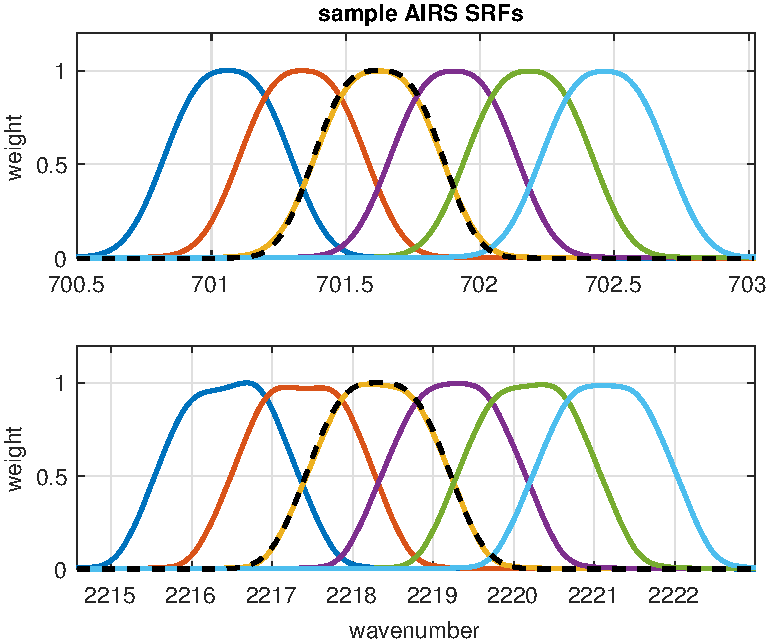
\includegraphics[width=\linewidth]{figures/airs_sample_SRF.pdf}
  \caption{Sample AIRS spectral response functions from the low
    and high ends of the band.  The dashed line is a generalized
    Gaussian function.}
  \label{srfs1}
\end{figure}

\begin{figure} % source plot_SRF2.m
  \centering
  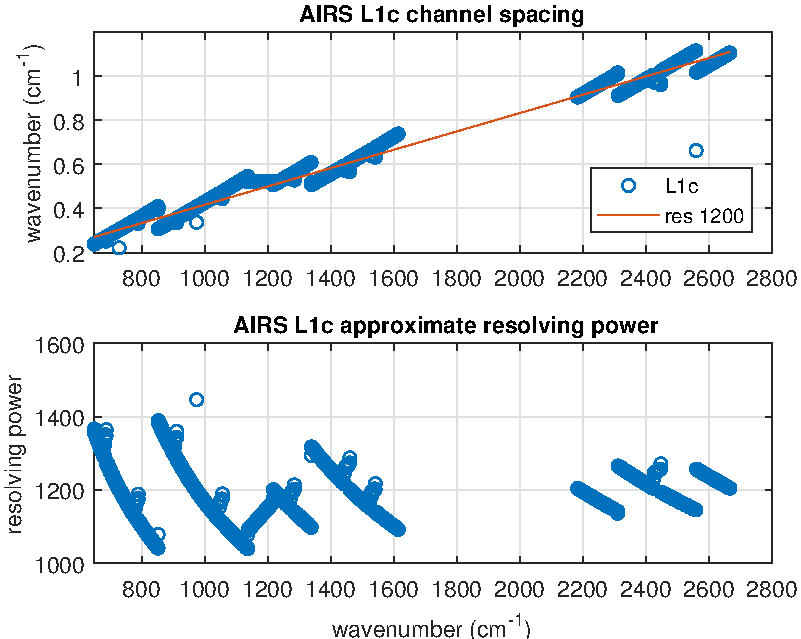
\includegraphics[width=\linewidth]{figures/airs_L1c_res.pdf}
  \caption{AIRS L1c channel spacing and resolving power, $R =
    v_i/\fwhm_i$.  The relatively regular L1c channel spacing aids
    the deconvolution.}
  \label{chan1}
\end{figure}

Figure \ref{srfs1} shows typical {\airs} SRFs from the low and high
ends of the band.  Note the significant overlap in the wings.  This
allows the deconvolution to recover resolution beyond that of
the response functions considered individually.  The SRFs are not
necessarily symmetrical, especially at the high end of the band, due
to fringing from the AIRS entrance filters.  The dashed line on top of
the third SRF in each group is a fit for a generalized Gaussian
\cite{wiki:gauss} of the form
\[w(v, v_0, \fwhm) = 
\exp\left(-\left(\frac{(v - v_0)^2}{2s^2}\right)^p\right), \] where
$s=\fwhm / (2\sqrt{2}\,(\ln 2)^{1/(2p)})$.  Parameters $v$, $v_0$
and $\fwhm$ are frequency, desired channel center, and desired full
width half max.  We chose $p = 1.4$ to give an approximate match to
{\airs} SRFs, though without the variation or extended tails of the
measured \srf s.  We will use this analytic representation to
calculate reference truth for the deconvolution and in section
\ref{airsL1d} as the basis for an idealized grating model.

% with the same {\FWHM} and channel centers,

Figure \ref{chan1} shows channel spacing and resolving power for the
{\airs} L1c channel set \cite{a1c:atbd}.  The variable channel
spacing and resolving power are due to the modular structure of the
focal plane.  Although not entirely regular---that is, not a simple
function of frequency---the L1c channel set is more regular than the
L1b channel set from which it is derived, and we mainly consider the
L1c set here.

Suppose we have $n$ channels and a frequency grid $\vec v$ of $k$
points spanning the union of the domains of the functions
$\sigma_i$.  The grid step size for our applications is often 0.0025
{\wn}, the default resolution for upwelling radiances calculated
using the kCompressed Atmospheric Radiative Transfer Model (\kcarta)
\cite{kcarta1}.  Let $S_k$ be an $n\times k$ array such that
$s_{i,j} = \sigma_i(v_j)/w_i$, where $w_i = \sum_j \sigma_i(v_j)$,
that is where row $i$ is $\sigma_i(v)$ tabulated at the grid $\vec
v$ and normalized so the row sum is 1.  If the channel centers are
in increasing order $S_k$ is banded, and if they are not too close
(as is the case for a few of the L1b channels) the rows are linearly
independent.  $S_k$ is a linear transform whose domain is radiance
at the grid $\vec v$ and whose range is channel radiances.  If $r$
is radiance at the grid $\vec v$, then $c = S_k r$ gives a good
approximation of the channel radiances $c_i =
\int\sigma_i(v)r(v)\,dv$.  In practice this is how we calculate
{\airs} channel radiances for the validation tests described in
subsequent sections.

% We construct $S_k$ either explicitly or implicitly from the
% {\airs} {\srf} tabulations.  The matrix $S_k$ in the former case
% is large but manageable with a banded or sparse representation.

For the {\airs} to {\cris} and other translations we are mainly
interested in the transform $S_b$ for {\srf}s at an intermediate
resolution, typically $0.1~\wn$.  This is the approximate resolution
of the {\srf} measurements and convenient for reconvolution to the
{\cris} user grid.  So let $\vec v_b = v_1,v_2,\ldots,v_m$ be a
$0.1~\wn$ grid spanning the domains of the functions $\sigma_i$.
Similar to $S_k$, let $S_b$ be an $n\times m$ array where row $i$ is
$\sigma_i(v)$ tabulated at the $\vec v_b$ grid, with rows normalized
to~1.  If $r$ is radiance at the $\vec v_b$ grid, then $c = S_b r$
is still a reasonable approximation of $\int\sigma_i(v)r(v)\,dv$.

For our application we want to start with $c$ and find $r$, that is
to deconvolve $c$ by solving $S_b r = c$ for $r$.  Since $n < m$,
the system is underdetermined.  We take the Moore-Penrose
pseudoinverse \cite{wiki:pinv, strang:linalg} of $S_b$ to get $r_0 =
S_b^{-1} c$.  This gives a minimal solution, in the sense that
$||r_0||_2 \le ||r_j||_2$ for all $r_j$ satisfying $S_b r_j = c$.
The condition number for $S_b$ as built from the L1c channels is
$||S_b||_2||S_b^{-1}||_2 = 115$, which is tolerable.\footnote{The
  notation $||S||_2$ is the $L^2$ norm of $S$, and is simply
  Euclidian distance for vectors.\cite{wiki:norm}.}

Although our main goal is to reconvolve the deconvolved {\airs}
radiances to the {\cris} or other user grids, as a check we first
compare the deconvolved radiances with reference truth from a direct
convolution of {\kcarta} radiance to the $0.1~\wn$ grid.  The
response function we use for this is the generalized Gaussian above
with ${\fwhm} = v_i / 2000$, where $v_i$ are the grid frequencies.
This represents a hypothetical grating spectrometer with a resolving
power of 2000, oversampled to the 0.1~\wn\ grid.

% The choice of basis functions for a deconvolution reference truth is
% perhaps not obvious, since the deconvolution is undoing---at least
% to some extent---the effects of the {\airs} SRF convolutions.

% The value of 2000 was chosen to give an approximate fit to the
% deconvolved radiances.  We also tried a generalized Gaussian with a
% fixed {\FWHM} for values $0.4$, $0.6$, and $0.8$ and a sinc basis
% with a spacing of $0.2$~\wn, all of which gave larger residuals.

\begin{figure} % source decon_test1.m
  \centering
  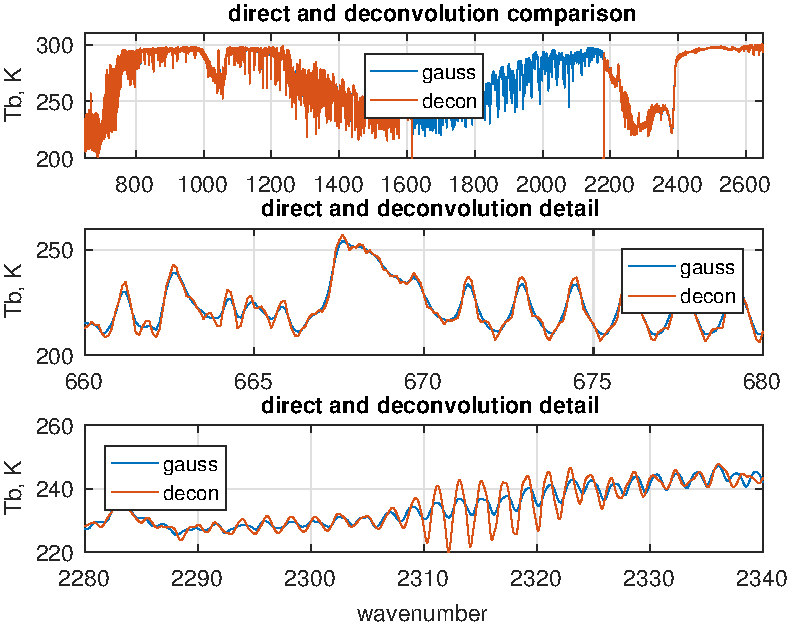
\includegraphics[width=\linewidth]{figures/airs_decon_spec.pdf}
  \caption{Spectra from fitting profile 1 for deconvolved AIRS
    and the reference convolution to the $0.1$~\wn\ grid.  We see
    some overshoot and ringing in the deconvolution.}
  \label{dspec}
\end{figure}

\begin{figure} % source decon_test1.m 
  \centering
  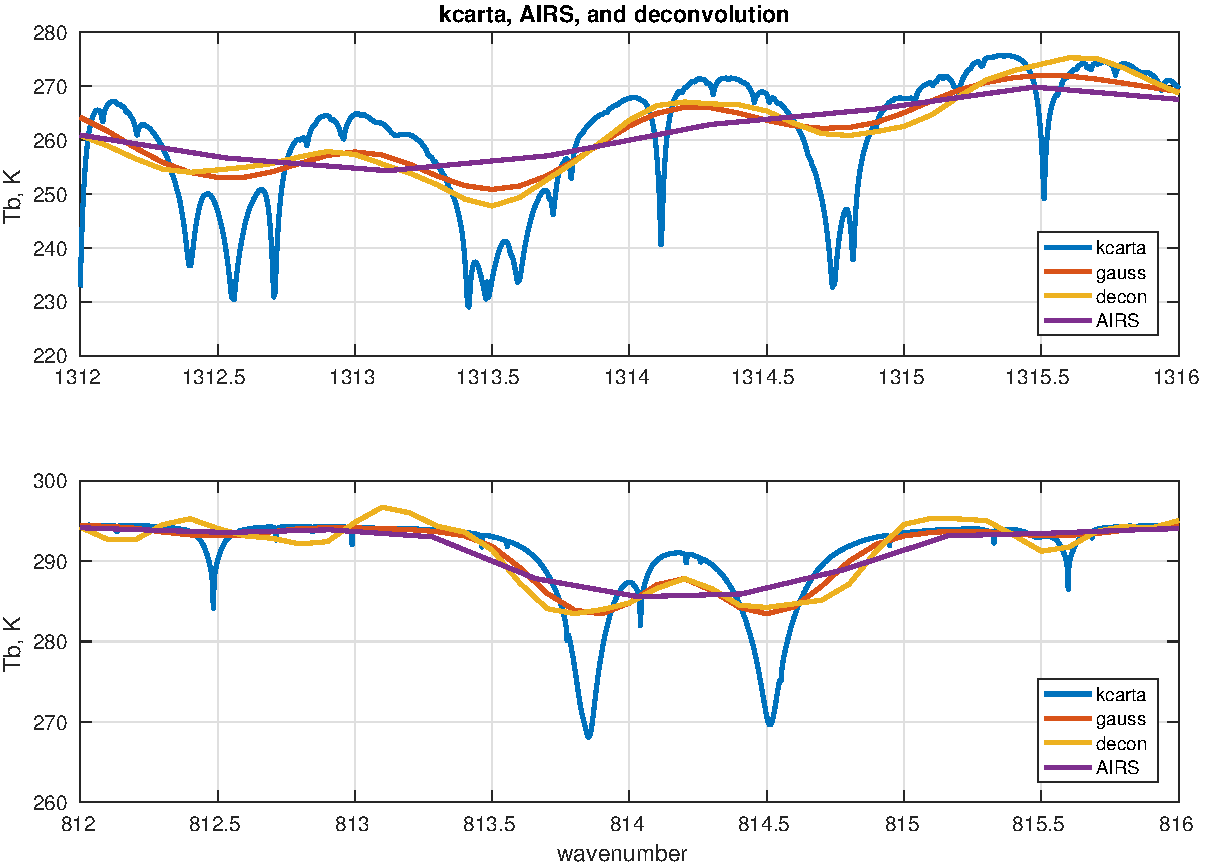
\includegraphics[width=\linewidth]{figures/airs_decon_zoom.pdf}
  \caption{Details from fitting profile 1 for {\kcarta}, the
    reference convolution to the $0.1$~\wn\ grid, deconvolved
    AIRS, and true AIRS.  The deconvolution restores some
    detail.}
  \label{dzoom}
\end{figure}

\begin{figure} % source plot_Binv.m
  \centering
  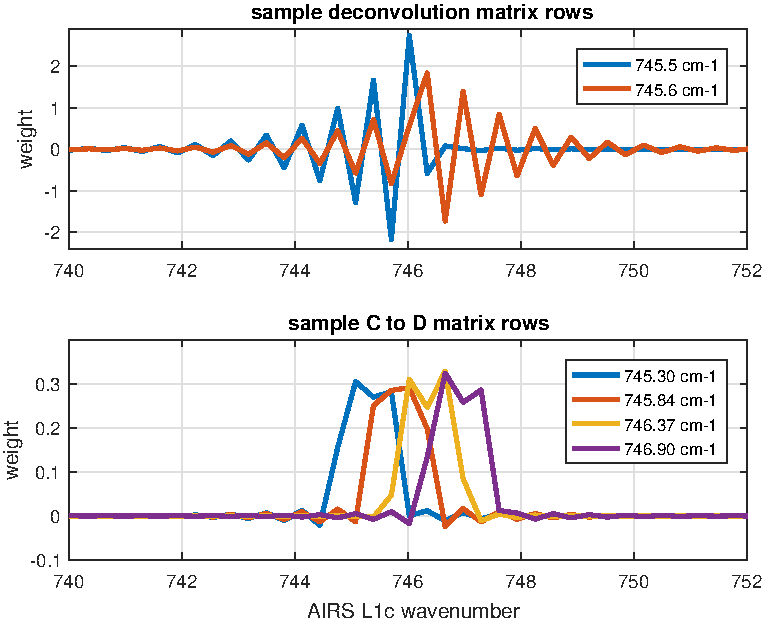
\includegraphics[width=\linewidth]{figures/airs_decon_basis.pdf}
  \caption{Sample adjacent rows for the deconvolution and L1c to L1d
    transforms}
  \label{dbasis}
\end{figure}

The {\airs} deconvolution gives a modest resolution enhancement, at
the cost of added artifacts and noise.  Figure \ref{dspec} shows
spectra from fitting profile~1 \cite{sarta1,sarta2} for the {\airs}
deconvolution together with reference truth, with sample details
from the low and high ends of the band.  The ringing or overshoot at
2310~{\wn} is due to a change in the L1c channel spacing from
1.02~{\wn} to 0.92~{\wn} at that point.
% These changes occur at the AIRS focal plane module boundaries.
% The first subplot of Figure \ref{chan1} shows channel spacing as a
% function of frequency, and we see the jump at 2310~{\wn} is one of
% several such discontinuities.
Figure \ref{dzoom} shows details of {\kcarta}, the reference
convolution, deconvolution, and AIRS spectra for fitting profile~1.
In the first subplot we see the deconvolution is capturing some of
the fine structure in the {\kcarta} data that is present in the
reference convolution but not the AIRS data.  In the second subplot
we see the deconvolution (and reference convolution) resolving a
pair of close lines that are not resolved at the {\airs} L1c
resolution.  But we also see some ringing that is not present in the
reference convolution.  This is to be expected; significant detail
is lost in the convolution to {\airs} channel radiances and this can
only partially be recovered by the deconvolution.  The artifacts are
acceptable because we do not propose using the deconvolved radiances
directly; they are an intermediate step before reconvolution to a
lower resolution.

% \begin{figure} % source decon_test1.m
%   \centering
%   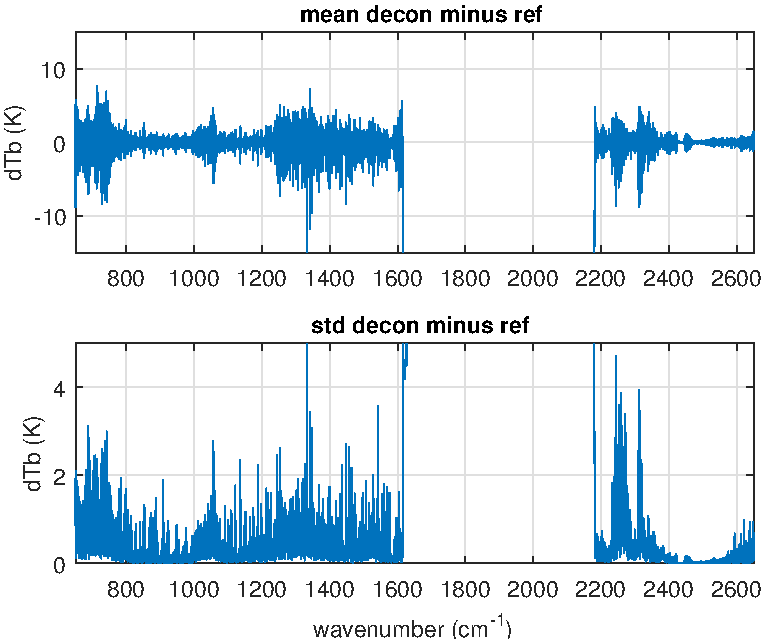
\includegraphics[width=\linewidth]{figures/airs_decon_diff.pdf}
%   \caption{mean and standard deviation over the 49 fitting profiles
%     for the L1c deconvolution minus direct convolution to the
%     $0.1$~\wn\ intermediate grid.  The residuals are too large to use
%     the deconvolved radiances directly.}
%   \label{ddiff}
% \end{figure}

% Figure \ref{ddiff} shows the mean and standard deviation of the
% difference of the deconvolved minus the directly convolved radiances
% for all 49 fitting profiles.  The residuals are large but mainly
% significant for understanding limitations of the deconvolution.
% The residuals can be reduced dramatically by reconvolving the
% $0.1$~\wn\ intermediate grid to a lower resolution.  We consider
% this for convolution to the {\cris} user grid in the next section.

Figure \ref{dbasis} shows a pair of typical adjacent rows of the
deconvolution matrix $S_b^{-1}$\, in the first subplot.  Row $i$ of
$S_b^{-1}$ is the weights applied to L1c channel radiances to
synthesize the deconvolved radiance $r_i$ at the intermediate grid
frequency $v_i$.  The oscillation shows we are taking the closest
AIRS channel, subtracting weighted values for channels $\pm 1$ step
away, adding weighted values for channels $\pm 2$ steps away, and so
on, with the weights decreasing quickly as we move away from $v_i$,
with eight to ten L1c channels making a significant contribution to
each deconvolution grid point.  The second subplot shows four
adjacent rows of the matrix $S_d \cdot S_b^{-1}$, which takes L1c to
L1d channel radiances.  (The L1d radiances are discussed in a later
section; here they are of interest mainly as a typical
reconvolution.)  Both matrices are banded but the bands are narrower
in the second, with three to five L1c channels contributing to each
L1d channel.  This span of influence gives us the set of parents for
each translated channel.

%---------------------------------------------------------------------
% \FloatBarrier
\section{AIRS to CrIS translation}
\label{airs2cris}

Given {\airs} deconvolution to a $0.1~\wn$ intermediate grid,
reconvolution to the {\cris} user grid is straightforward.  For
{\cris} standard resolution the channel spacing is $0.625~\wn$ 
for the LW band, $1.25~\wn$ for the MW, and $2.5~\wn$ for the SW.
For each {\cris} band, we (1)~find the {\airs} and {\cris} band
intersection, (2) apply a bandpass filter to the deconvolved {\airs}
radiances restricting them to the intersection, with a rolloff
outside the passband, and (3) reconvolve the filtered spectra to 
the {\cris} user grid with a zero-filled double Fourier transform
\cite{git:finterp}.  The out-of-band rolloff smooths what would
otherwise be an impulse at the band edges, reducing ringing in the
translation.  

Translations are tested by comparison with calculated reference
truth.  We start with a set of atmospheric profiles and calculate
upwelling radiance at a $0.0025~\wn$ grid with {\kcarta}
\cite{kcarta1} over a band spanning the domains of the {\airs} and
{\cris} response functions.  ``True {\airs}'' is calculated by
convolving the {\kcarta} radiances with {\airs} SRFs and ``true
{\cris}'' by convolving {\kcarta} radiances to a sinc basis at the
{\cris} user grid.  True {\airs} is then translated to {\cris} to
get ``{\airs} {\cris}'', and this is compared with true {\cris}.
Figure~\ref{specLW} shows sample spectra for true {\airs},
deconvolved {\airs}, true {\cris} and {\airs} {\cris}.  Any
difference between true {\cris} and {\airs} {\cris} is hard to see
here, and in subsequent plots we mainly show explicit differences.

Comparisons are done both with and without apodization.  Hamming
apodization \cite{barn2000, wiki:wind} sacrifices some resolving
power but gives a significant reduction in the residuals and is
convenient for many applications.  Convolution, deconvolution, and
apodization are done with radiances, while spectra are presented and
statistics are done after conversion to brightness temperatures.

\begin{figure} % source a2cris_test1
  \centering
  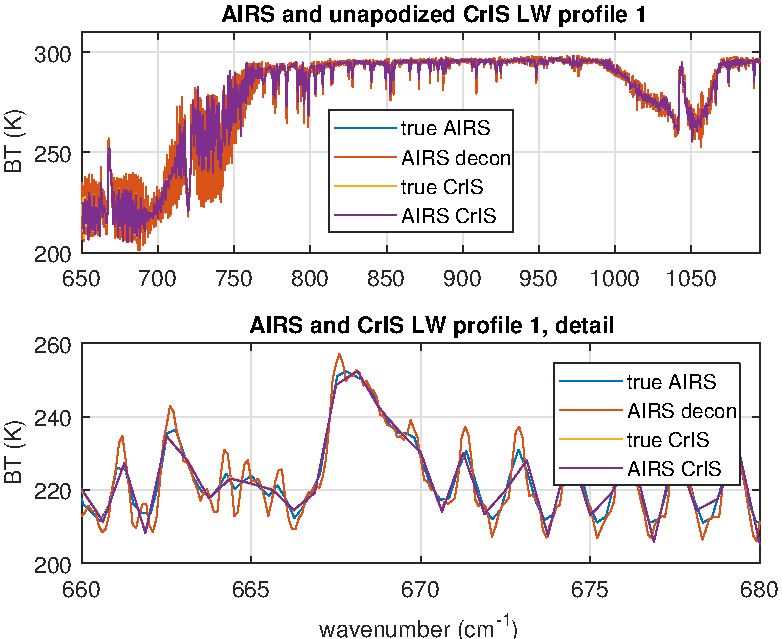
\includegraphics[width=\linewidth]{figures/a2cris_spec_LW.pdf}
  \caption{True AIRS, deconvolved AIRS, true CrIS, and AIRS CrIS.
    Differences between true CrIS and AIRS CrIS are too small to be
    visible in this figure.}
  \label{specLW}
\end{figure}

\begin{figure} % source a2cris_test1
  \centering
  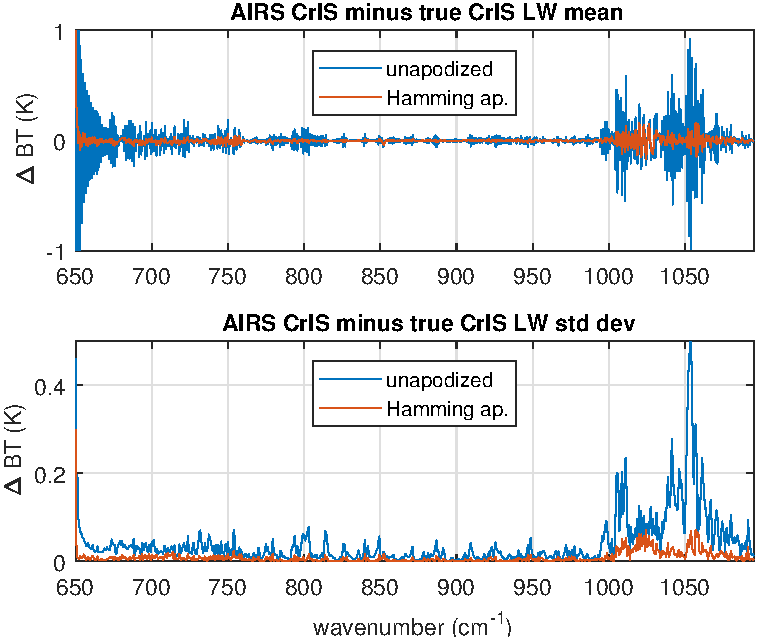
\includegraphics[width=\linewidth]{figures/a2cris_diff_LW.pdf}
  \caption{Mean and standard deviation of unapodized and Hamming
    apodized AIRS CrIS minus true CrIS, for the LW band.}
  \label{diffLW}
\end{figure}

\begin{figure} % source a2cris_test1
  \centering
  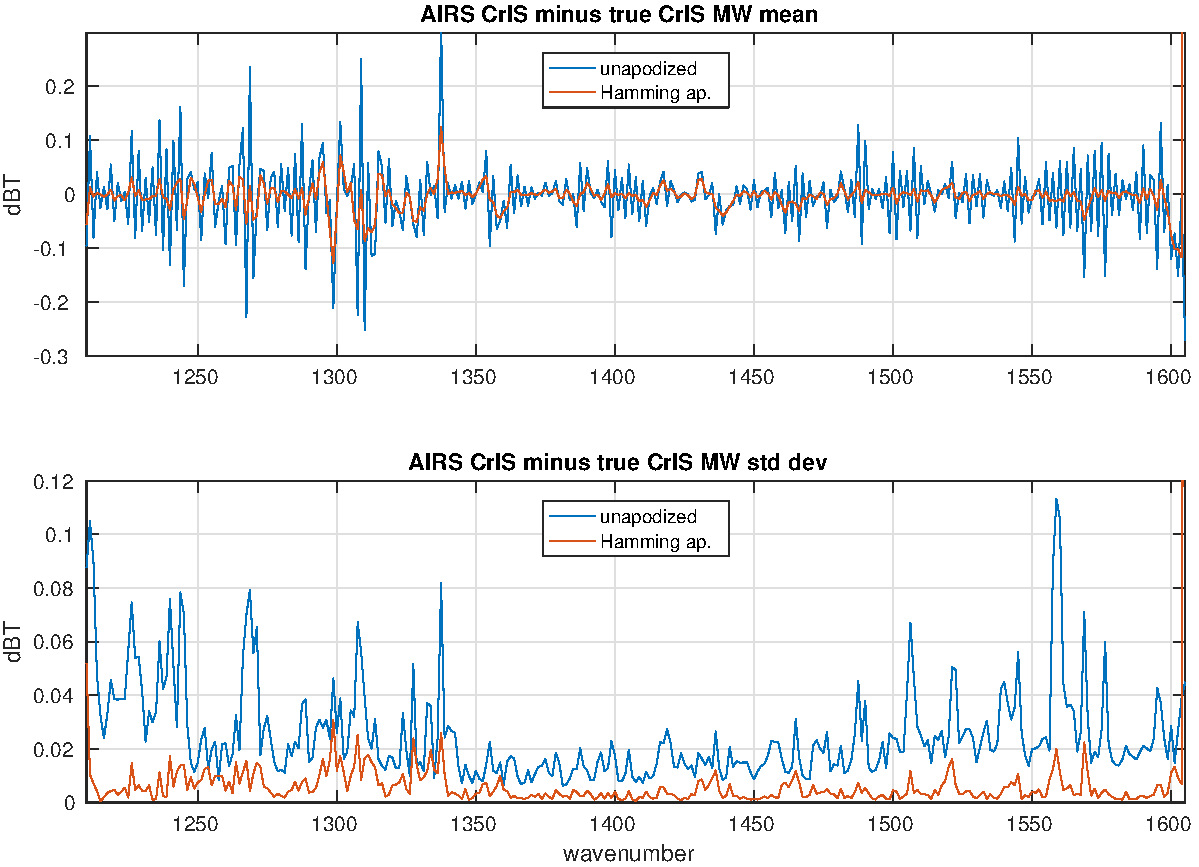
\includegraphics[width=\linewidth]{figures/a2cris_diff_MW.pdf}
  \caption{Mean and standard deviation of unapodized and Hamming
    apodized AIRS CrIS minus true CrIS, for the MW band.}
  \label{diffMW}
\end{figure}

\begin{figure} % source a2cris_test1
  \centering
  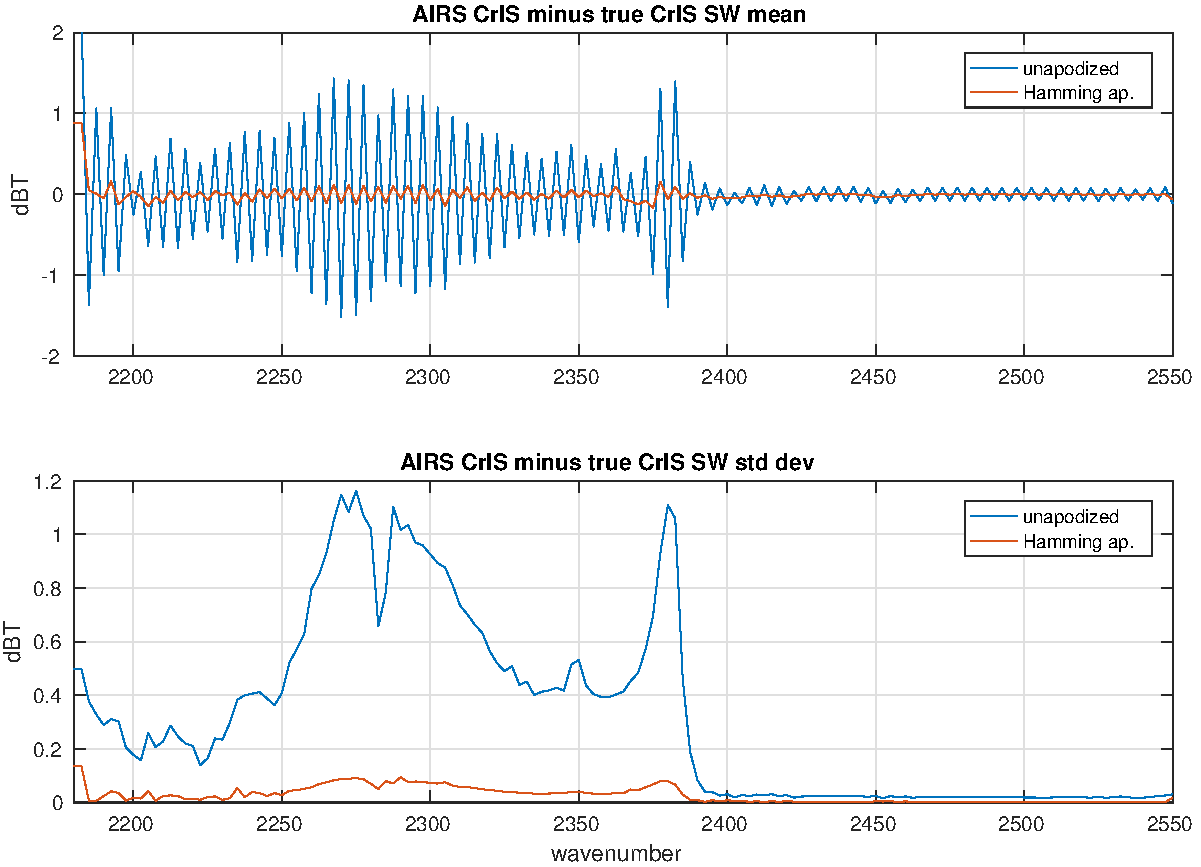
\includegraphics[width=\linewidth]{figures/a2cris_diff_SW.pdf}
  \caption{Mean and standard deviation of unapodized and Hamming
    apodized AIRS CrIS minus true CrIS, for the SW band.}
  \label{diffSW}
\end{figure}

\begin{figure} % source a2cris_test1
  \centering
  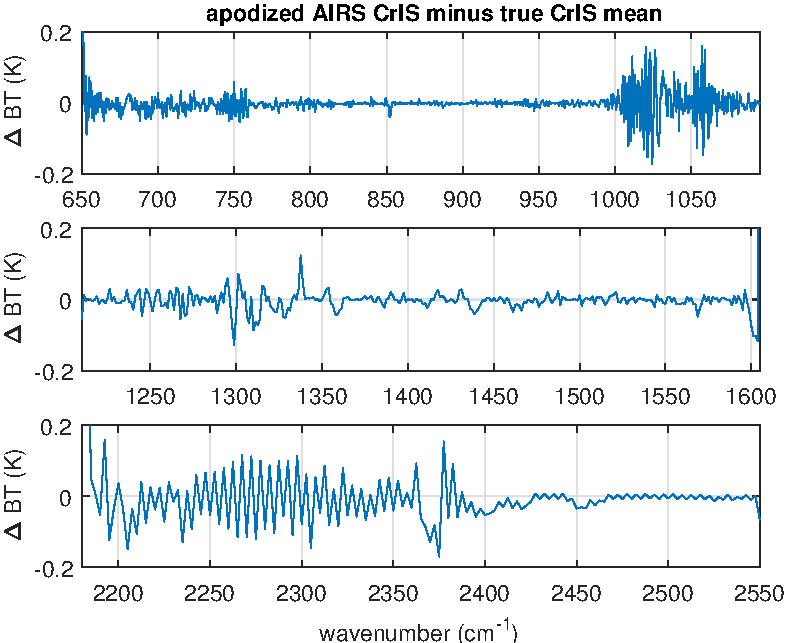
\includegraphics[width=\linewidth]{figures/a2cris_diff_all.pdf}
  \caption{Summary plot of the mean of apodized residuals for all
    three CrIS bands, showing the residuals in greater detail.}
  \label{meanAll}
\end{figure}

We use radiance from a set of 49 fitting profiles spanning a wide
range of clear atmospheric conditions as our test set, and as the
independent set for statistical sets.  This set was initially chosen
for testing radiative transfer codes \cite{sarta1,sarta2} and is
highly uncorrelated; reducing the reconstruction residual to 0.02~K
requires 48 left-singular vectors.  (Details of this correlation
measure are given in an appendix.)  For regression tests we use
radiance from a set of 7377 all-sky (clear and cloudy) AIRS profiles
spanning several consecutive days as our dependent set.  This set is
more correlated; reducing the reconstruction residual to 0.02~K
requires 260 left-singular vectors.  We did try splitting the 7377
profile set into dependent and independent subsets.  Residuals from
this larger independent set were consistently smaller than from the
49-profile set, suggesting the latter makes for a stricter test.

Figures \ref{diffLW}, \ref{diffMW}, and \ref{diffSW} show the mean
and standard deviation of true {\cris} minus {\airs} {\cris} for the
49 fitting profiles, for each {\cris} band.  The Hamming apodization
gives a significant reduction in the residuals.  Figure
\ref{meanAll} summarizes results all three bands, for apodized
radiances.  The constant or DC bias is very close to zero for the
apodized residuals.  Both the apodized and unapodized residuals are
significantly less than the corresponding residuals from
conventional interpolation, as shown in the appendix.

% $0.002$~K for the LW, $-0.005$~K for the MW, and $0.001$~K for 
% the SW.

% At the low end of the {\cris} LW band there are only the two
% {\airs} ``guard channels'' below 650 {\wn}, so the rolloff is
% abrupt and we have significant ringing in the translation.

The relatively small standard deviation of the residuals suggests
some regularity, and we can see an oscillation with a period of two
channel steps in several places.  Up to this point there has been no
statistical component to our translation, beyond the choice of test
set for validation.  We feel it is important to be clear about any
steps that require statistical fitting.  That said, we can use a
simple linear correction for a significant further reduction of the
residuals.  We use the set of 7377 mostly cloudy AIRS profiles as
the dependent set and the 49 profile set as the independent or test
set.

We compare three such corrections.  These are done with a separate
regression for each {\cris} channel, and so introduce no
cross-correlations.  Let $\Ttc_i$ be true {\cris} and $\Tac_i$
{\airs} {\cris} brightness temperatures for {\cris} channel $i$,
from the dependent set.  For the bias test we subtract the mean
residual from the dependent set.  For the linear test we find $a_i$
and $b_i$ to minimize $||a_i\,\Tac_i + b_i - \Ttc_i||_2$, and for
the quadratic test weights $c_i$, $a_i$ and $b_i$ to minimize
$||c_i\,(\Tac_i)^2 + a_i\,\Tac_i + b_i - \Ttc_i||_2$.  The resulting
correction is then applied to the independent set, the 49 fitting
profiles, for comparison with true {\cris}.

Figure \ref{statLW} is a comparison of bias, linear, and quadratic
corrections for the LW band.  The linear and quadratic corrections
are nearly identical, with the quadratic coefficient very close to
zero.  Figure \ref{coefLW} shows the weights for the linear fits
from figure \ref{statLW}.  The $a$ weights are very close to 1 and
the $b$ weight to the bias.  Figures \ref{statMW} and \ref{statSW}
show the linear correction giving a similar improvement in the MW
and a small improvement in the SW, where the quadratic correction is
noticably worse.  Figure \ref{statAll1} shows the residuals for the
apodized linear correction for all three bands.  The residuals are
significantly reduced in comparison with the apodized uncorrected
radiances shown in figure \ref{meanAll} and are generally less than
NEdT (for the first fitting profile), as we show next.

\begin{figure} % source a2cris_regr2.m
  \centering
  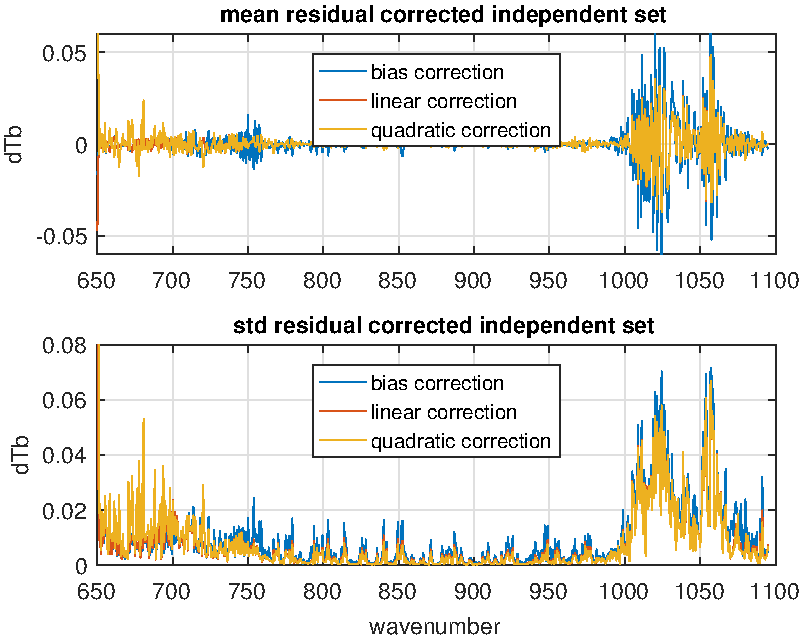
\includegraphics[width=\linewidth]{figures/a2cris_regr_LW.pdf}
  \caption{Mean and standard deviation of corrected apodized AIRS
    CrIS minus true CrIS, for the LW band.}
  \label{statLW}
\end{figure}

\begin{figure} % source a2cris_regr2.m
  \centering
  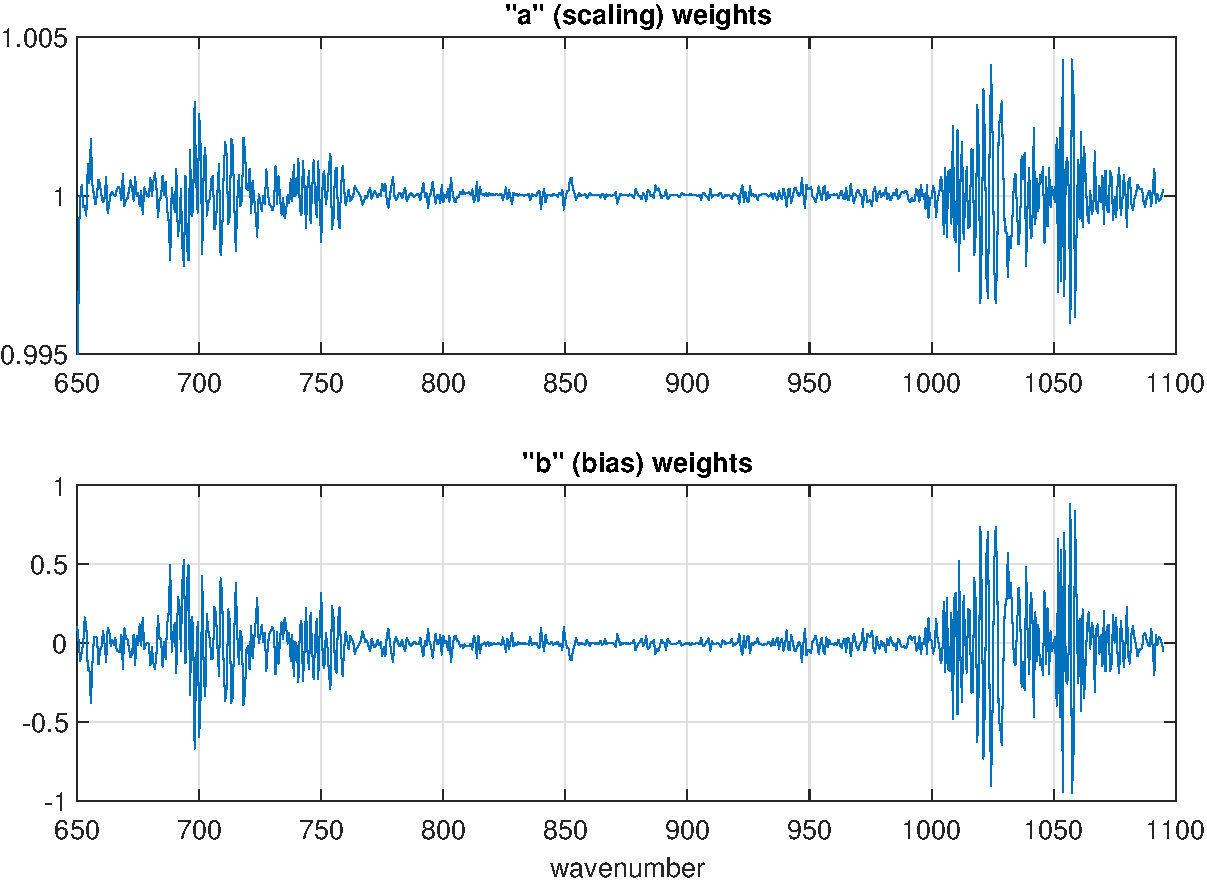
\includegraphics[width=\linewidth]{figures/a2cris_coef_LW.pdf}
  \caption{Weights for the linear correction $ax+b$, for the LW
    band.}
  \label{coefLW}
\end{figure}

\begin{figure} % source a2cris_regr2.m
  \centering
  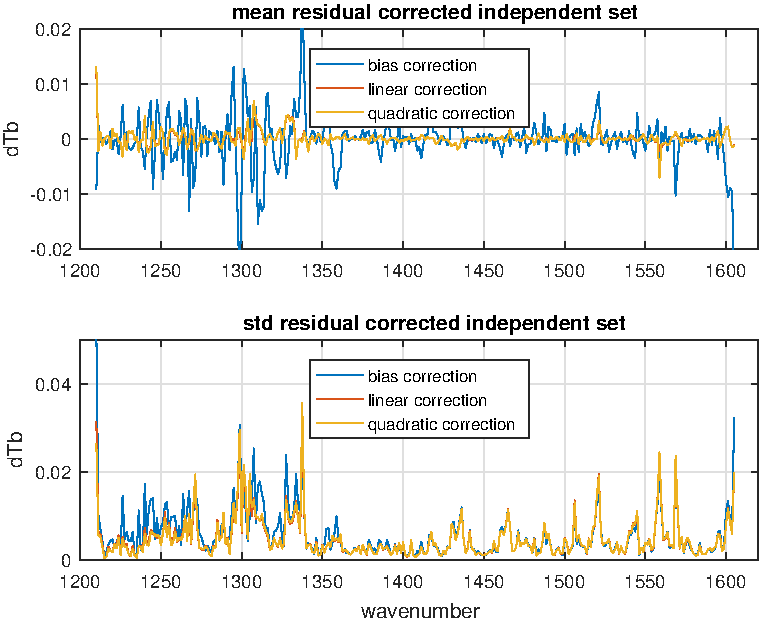
\includegraphics[width=\linewidth]{figures/a2cris_regr_MW.pdf}
  \caption{Mean and standard deviation of corrected apodized AIRS
    CrIS minus true CrIS, for the MW band.}
  \label{statMW}
\end{figure}

\begin{figure} % source a2cris_regr2.m
  \centering
  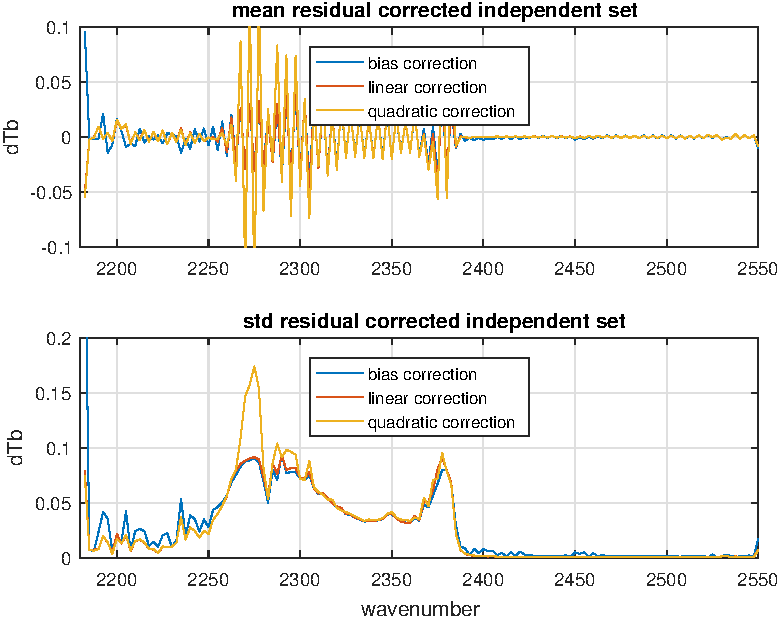
\includegraphics[width=\linewidth]{figures/a2cris_regr_SW.pdf}
  \caption{Mean and standard deviation of corrected apodized AIRS
    CrIS minus true CrIS, for the SW band.}
  \label{statSW}
\end{figure}

\begin{figure} % source a2cris_test2.m
  \centering
  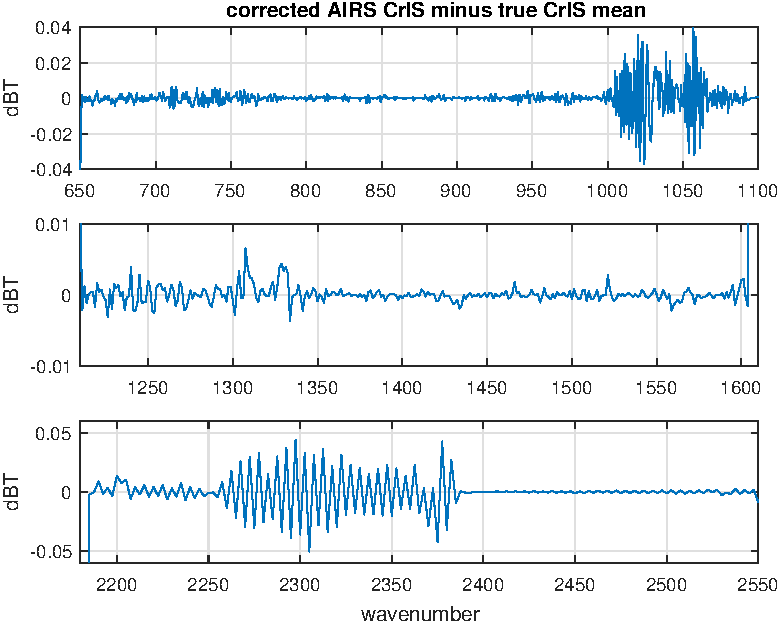
\includegraphics[width=\linewidth]{figures/ap_decon_corr.pdf}
  \caption{Mean corrected apodized residuals for all three bands,
    showing the linear corrected apodized residuals in greater
    detail.}
  \label{statAll1}
\end{figure}

% \begin{figure} % source a2cris_test2.m
%   \centering
%   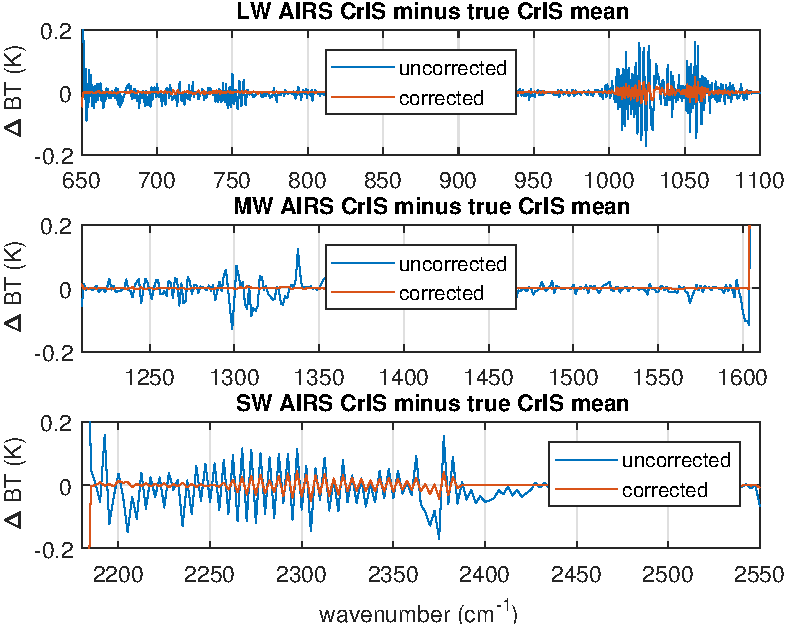
\includegraphics[width=\linewidth]{figures/a2cris_regr_all.pdf}
%   \caption{Mean corrected and uncorrected apodized residuals for all
%     three bands.}
%   \label{statAll2}
% \end{figure}

\begin{figure} % source nedn_test2.m
  \centering
  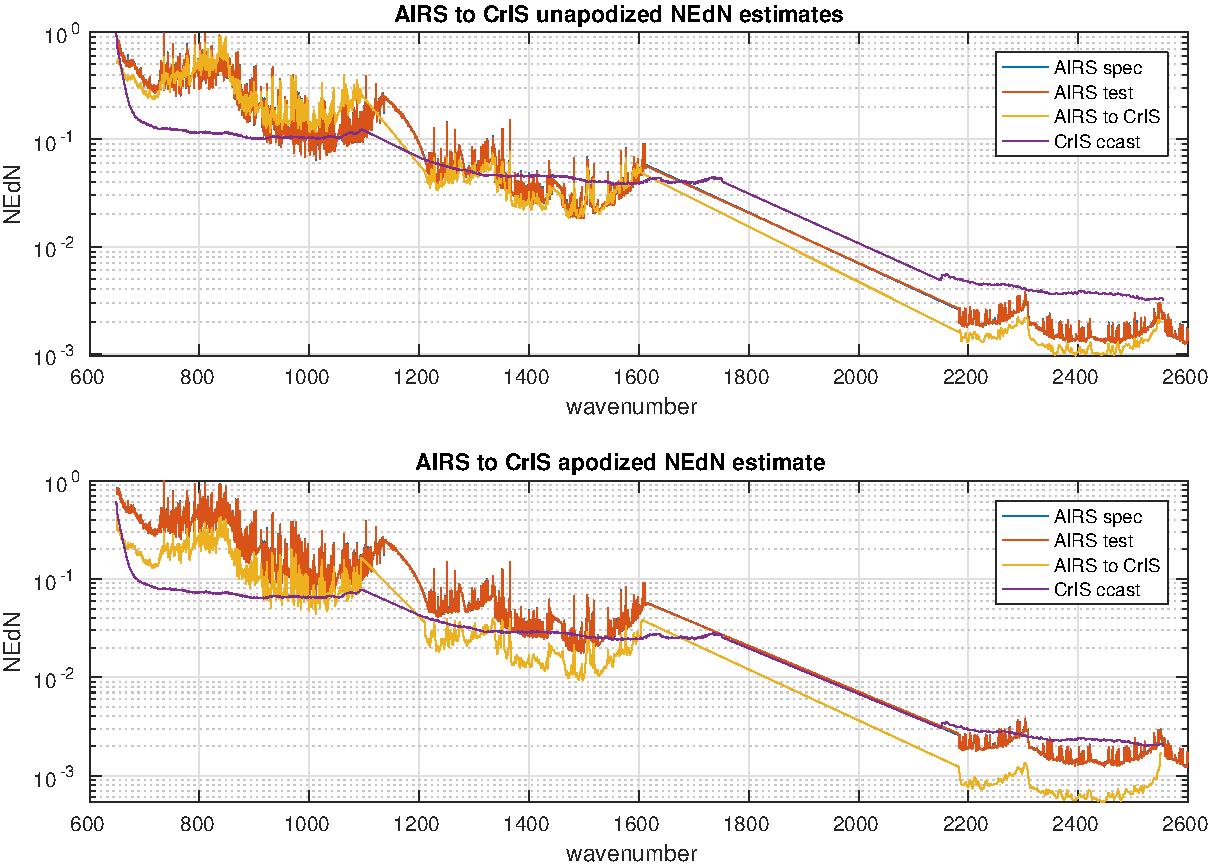
\includegraphics[width=\linewidth]{figures/a2cris_nedn.pdf}
  \caption{AIRS, AIRS-to-CrIS, and CrIS NEdN.
    Apodization reduces the CrIS and AIRS-to-CrIS NEdN by a
    factor of $0.63$.}
  \label{nedn}
\end{figure}

\begin{figure} % source nedt_test1.m
  \centering
  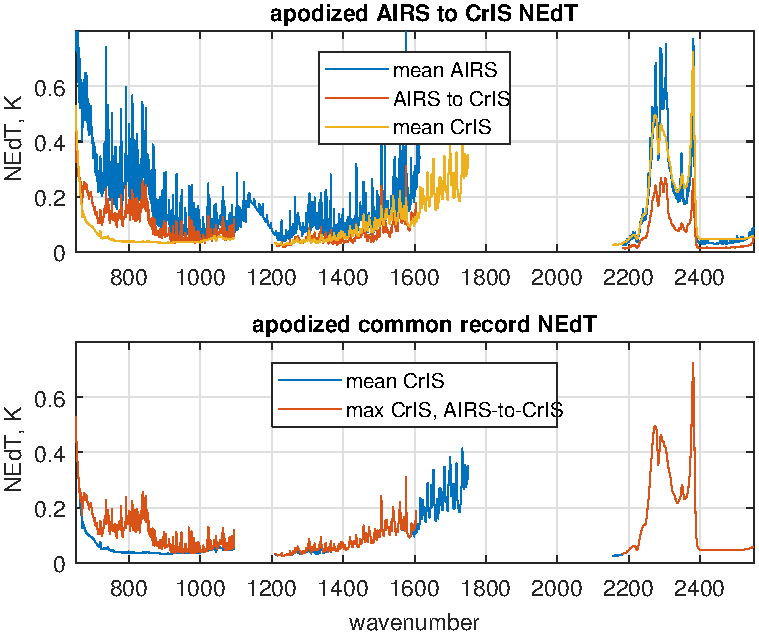
\includegraphics[width=\linewidth]{figures/a2cris_nedt.pdf}
  \caption{AIRS, AIRS-to-CrIS, and CrIS apodized NEdT,
    and the max of CrIS and AIRS-to-CrIS NEdN (shown as
    NEdT) with CrIS NEdT shown as a reference.}
  \label{nedt}
\end{figure}

We can give a good estimate of noise equivalent differential
radiance (NEdN) for the translation by adding noise with a normal
distribution at the {\airs} NEdN to blackbody radiance at 280K,
translating this to {\cris}, and measuring the noise of the
translation.  Figure \ref{nedn} shows the measured
{\airs}-to-{\cris} NEdN together with {\airs} and {\cris} NEdN for
both apodized and unapodized radiances.  The {\airs} and {\cris}
values are averages over a full day, 4 Dec 2016.  NEdN for the L1c
synthetic channels is interpolated.  The first subplot of figure
\ref{nedt} is NEdT for apodized radiances, for fitting profile 1.
The translation to apodized {\cris} reduces NEdN significantly for
all three bands.  Translation to unapodized {\cris} reduces NEdN
slightly for the MW and SW bands, while LW NEdN is similar up to
about 900 cm-1 and then a little higher past that.

% correlation for L1c synthetic channels, and channels with more
% than one L1b parent, may not be well-defined.

Our modeling with normally distributed noise does not take into
account potential correlation of the {\airs} noise.  The AIRS L1b
data does have some noise correlation, mainly within modules.  The
question of correlation becomes more complex with the translation to
L1c.  In contrast {\cris} instrument noise is largely uncorrelated.
The effect of the deconvolution-based translation is similar to a
mild apodization, and so should have a generally similar effect on
the correlated component of {\airs} noise.  Since we are reducing
NEdN in the translation (except for the LW unapodized case), it
seems unlikely we are increasing problems with the correlated
component, except perhaps relative to the reduced NEdN.  But to
prove that we’d need a plausible model of L1c noise correlation,
which we do not have at the present time.

% The sources of such noise might be vibration, radiation, or any
% common-mode effect.  Details concerning correlation sources are
% beyond the scope of this paper, except to note that noise for L1c
% channels with more than one L1b parent may not be well-defined.  In
% practice this is a relatively small set that we may want to use with
% caution.

The {\airs} channel-to-channel NEdN variation is significant; in the
upper half of the LW and most of the MW it is of the same order as
the {\airs} and {\cris} NEdN difference.  This variation is due the
{\airs} focal plane structure and sensitivity.  The {\airs} and
{\cris} NEdN measures are both spiky when averaged over a few
minutes but the {\cris} variation is primarily uncertainty in the
noise measurement and smooths out as the time span is extended,
while the {\airs} variation is stable.  The {\airs}-to-{\cris}
translation inherits this variability; it is a significant part of
the difference between {\airs} {\cris} and true {\cris}.  For a
common record we might want to add noise on a channel-by-channel
basis to whichever NEdN value---{\airs} {\cris} or true {\cris}---is
lower.  NEdN for the combined record would then be max of the
{\airs} {\cris} and true {\cris} NEdN values, as shown in the second
subplot of figure \ref{nedt}.

In addition to the standard resolution described above, in December
2014 {\cris} switched to a high resolution mode with a nominal
{\opd} of $0.8$~cm for all three bands, while continuing to support
the standard resolution product.  {\airs} does not have the
resolving power to properly support a translation to the {\cris}
high resolution MW and SW bands---the residuals for that case are
relatively large.  One solution for a common record might be a
compromise {\cris} resolution of $0.6$~cm for the MW and $0.4$~cm
for the SW, to roughly match the {\airs} resolving power.

As an alternative, in the next section we consider translation from
{\airs} to an idealized grating model.  For use as a common record
this would require translations from both {\airs} and {\cris}.  
The {\cris} high resolution mode allows for a {\cris} to {\airs}
translation, as described in \cite{git:decon}.  The residuals are
larger in the LW than for our translation from {\airs} to {\cris},
but may be acceptable for some applications.  A {\cris} translation
to the proposed idealized grating model should work at least as
well.

%---------------------------------------------------------------------
% \FloatBarrier
\section{Translation to an idealized grating model}
\label{airsL1d}

% The nominal {\airs} resolution is 1200, though for many modules
% the real resolving power is higher.

The {\airs} deconvolution can be used for other translations.  
In this section we briefly examine reconvolution to an idealized
grating model for resolving powers of 700 and 1200.  There are
several reasons to consider such a translation.  The constant
resolving power of the L1d basis (defined below) makes it a more
natural translation target for {\airs} than the constant channel
spacing of {\cris}.  It could be considered as the next step in
regularization of the {\airs} product, following the partial
regularization from L1b to L1c, and as a potential alternative
target for a long-term common record.

Define an {\airs} L1d basis with resolving power $R$ using the
generalized Gaussian response function of section \ref{decon} as
follows.  Let $v_0$ be the frequency of the first channel, and for
$i\ge0$, $\fwhm_i = v_i / R$, $dv_i = \fwhm_i / 2$, and $v_{i+1} =
v_i + dv_i$.  As with tests of the {\airs} to {\cris} translation,
true L1c is calculated by convolving {\kcarta} radiances with
{\airs} L1c SRFs and true L1d by convolving with an L1d basis at the
desired resolving power.  L1c is translated to L1d by deconvolution
followed by reconvolution to the desired L1d basis, and this is
compared with true L1d.

Figure \ref{L1d1200} shows residuals for reconvolution to an L1d
basis with resolving power of 1200, the nominal {\airs} resolution,
and figure \ref{L1d700s} shows residuals for a resolving power of
700.  Note the different x-axes for the two figures.  The residuals
depend in part on the L1d starting channel $v_0$, and so on how the
L1c and L1d SRF peaks line up.  The residuals shown are the result
of a rough fit for $v_0$.  For a resolving power of 1200 this gave
$v_0$ equal to the first L1c channel, while for 700 it was the first
L1c channel plus $0.2$~\wn.

We see that for both the {\airs} to {\cris} and L1c to L1d
translations some resolving power is sacrificed in shifting channel
centers to a single regular function of frequency.  Residuals for a
resolving power of 1200 (figure \ref{L1d1200}) are roughly
comparable to unapodized {\cris} (figures \ref{diffLW},
\ref{diffMW}, and \ref{diffSW}) and residuals for a resolving power
of 700 (figure \ref{L1d700s}) are roughly comparable to apodized
{\cris} (figure \ref{statAll1}).  As with the {\airs} to {\cris}
translation, the L1c to L1d residuals are significantly reduced with
a linear correction.  Residuals for L1d with a resolving power of
700 after correction are comparable to residuals for apodized
{\cris} after a similar correction.

\begin{figure} % source L1d_regr1.m
  \centering
  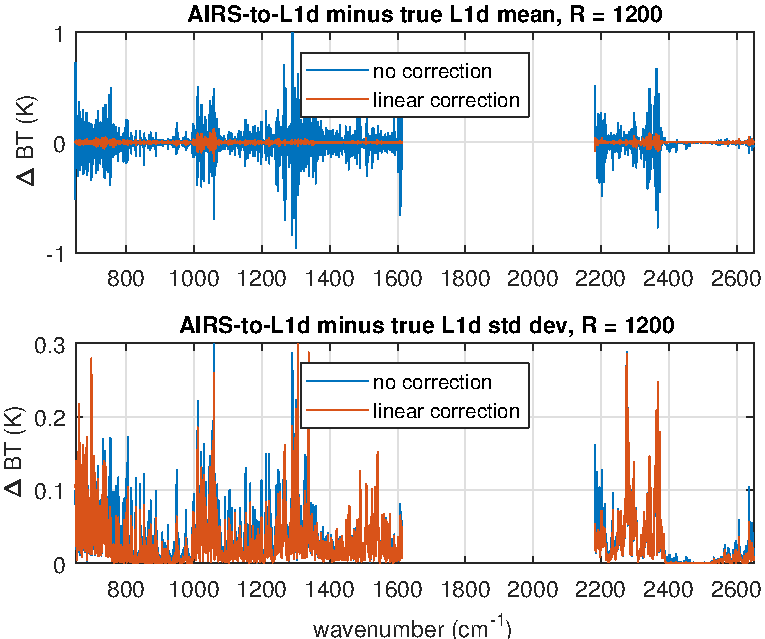
\includegraphics[width=\linewidth]{figures/L1d_cor1_1200.pdf}
  \caption{Mean and standard deviation for the AIRS L1c to L1d
    translation minus true L1d, for a resolving power of 1200.}
  \label{L1d1200}
\end{figure}

\begin{figure} % source L1d_regr1.m
  \centering
  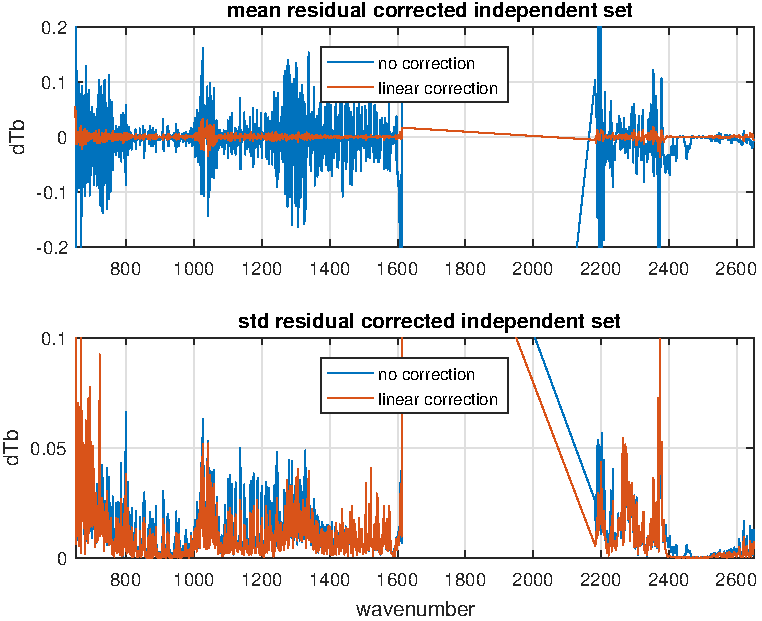
\includegraphics[width=\linewidth]{figures/L1d_cor1_700.pdf}
  \caption{Mean and standard deviation for the AIRS L1c to L1d
    translation minus true L1d, for a resolving power of 700.}
  \label{L1d700s}
\end{figure}

%---------------------------------------------------------------------
% \FloatBarrier
\section{Direct and principal component regression}
\label{dregr}

We want to compare our deconvolution-based translations with other
approaches to radiance translation, with an emphasis on methods we
have used in the past.  In this section we consider regression-based
translations, and in section \ref{interp} conventional
interpolation.

The {\airs} L1c to L1d translation can be done with a single 
linear transform $S_d\cdot S_c^{-1}$, where $S_c$ and $S_d$ are the
transforms taking the intermediate grid to L1c and L1d channels.
The {\airs} to {\cris} translation could also be done with a
composite transform if we use a resampling matrix rather than
double Fourier interpolation and a matrix form of the bandpass
filters.  We can get such a one-step tranform in other ways.
Suppose $r_a$ and $r_c$ are $m \times k$ and $n \times k$ {\airs}
and {\cris} radiance sets, for example true {\airs} and true {\cris}
from section \ref{airs2cris}.  We can find an $n \times m$ matrix
$X$ by regression to minimize $\|X r_a - r_c\|_2$ and use this as
our {\airs} to {\cris} transform.  We call this standard technique
``direct regression'' here.  This is different from the corrections
of section \ref{airs2cris} and \ref{airsL1d}; there regression was
used to find linear or quadratic correction coefficients
independently for each channel.

% Typically $k > m$, giving an apparently overdetermined
% system, and we solve $r_a^t X^t = r_c^t$ for $X$ by regression.

Figures \ref{dreg1} shows residuals for direct regression from
{\airs} to apodized {\cris} radiances.  As before we use the 7377
profile set as the dependent set and the 49 profile set as the
independent set.  The residuals are roughly comparable to the
residuals from the deconvolution translation summarized in figure
\ref{statAll1}.  However the regression matrices show significant
off-diagonal correlations.  Figure \ref{dreg3} shows this for the 
MW band; correlations are less for the LW and larger for the SW.  
In addition, the dependent set residuals are very small, much less
than the residuals for the independent set.  These are signs of
over-fitting.  As noted in section \ref{airs2cris} the 7377 profile
dependent set is highly correlated; the effective dimension (as
defined in the appendix) is only 260.

% The LW residual is larger at the low end of the band for direct
% regression and the high end for the deconvolved translation.
% Deconvolution does better in the MW, and direct regression in 
% the SW.

\begin{figure} % source a2cris_regr4X.m
  \centering
  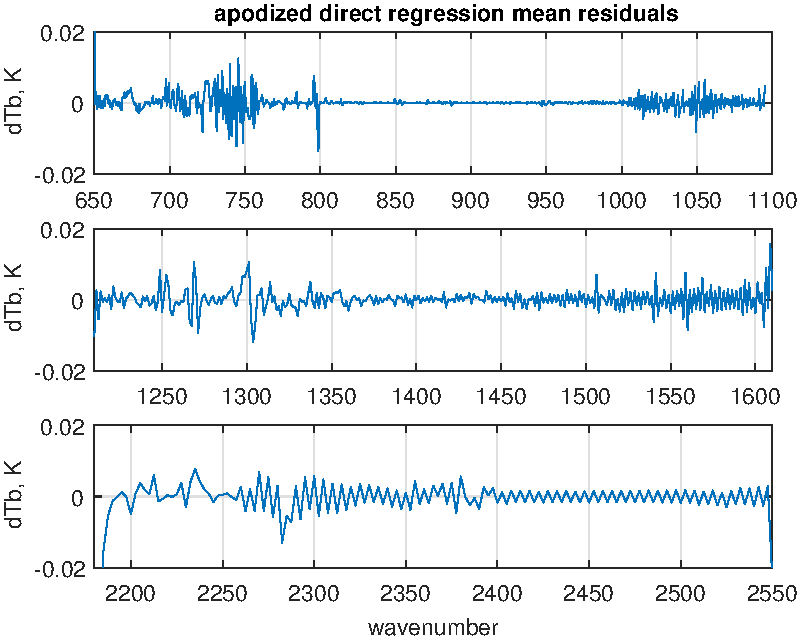
\includegraphics[width=\linewidth]{figures/ap_dir_regr.pdf}
  \caption{Mean residuals over the 49 profile independent set for
    AIRS to apodized CrIS direct regression.}
  \label{dreg1}
\end{figure}

\begin{figure} % source  a2cris_regr4X.m
  \centering
  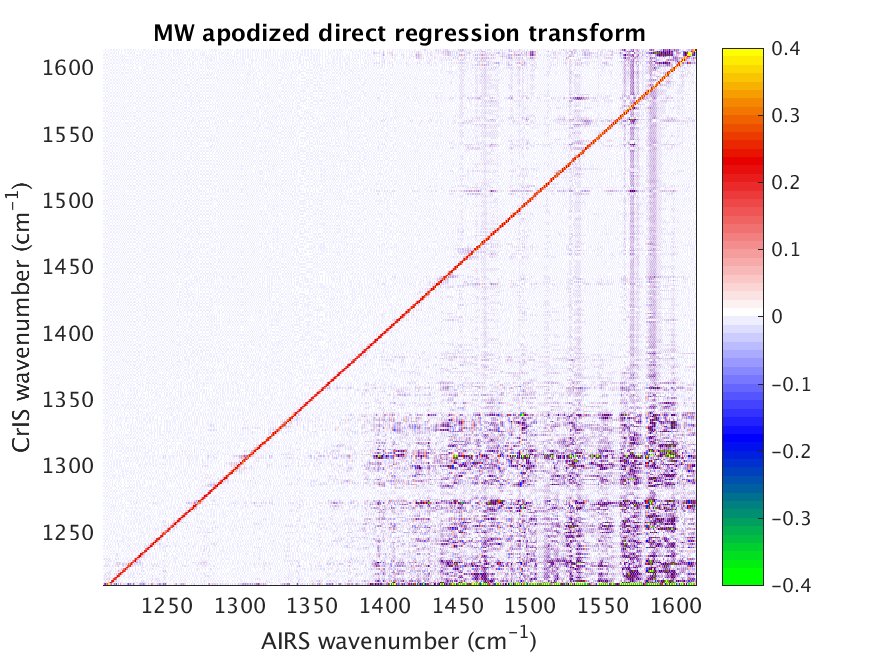
\includegraphics[width=\linewidth]{figures/MW_dir_regr_mat.png}
  \caption{Regression transform from the 7377 profile dependent set
    for the MW apodized direct regression transform.}
  \label{dreg3}
\end{figure}

% One fix is to add noise.  Recall that we generate true {\airs} 
% and true {\cris} by convolving a common set of high-resolution
% radiances.  For true {\airs} we can simply add noise at the {\airs}
% NEdN.  But for regression or testing of an {\airs} to {\cris}
% translation we want {\cris} radiances with actual translated {\airs}
% noise, not simply true {\cris} with noise added as per the {\cris}
% NEdN specification.  The latter does reduce correlations but
% increases residuals for the independent set significantly.
% To model NEdN for the {\airs} to {\cris} translation of section
% \ref{airs2cris} we synthesize noise at the {\airs} NEdN, add that 
% to the signal, run signal plus noise through the translation, and
% measure the noise.  But to get an {\airs} to {\cris} translation by
% regression with added noise we need a reference translation of each
% noisy {\airs} spectra.  We don't want to use the translation of
% section \ref{airs2cris} for that, at least not if our goal is to
% give each translation method an independent test.

\begin{figure} % source slackfigs a2cris_regr5.m
  \centering
  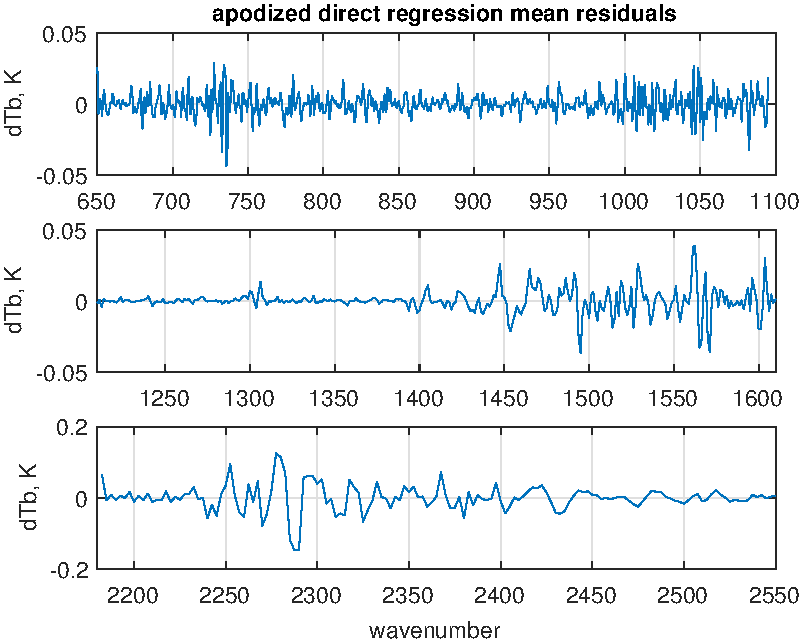
\includegraphics[width=\linewidth]{figures/ap_pc_regr.pdf}
  \caption{Mean residuals over the 49 profile independent set for
    AIRS to apodized CrIS principal component regression.}
  \label{dreg6}
\end{figure}

% \begin{figure} % source slackfigs a2cris_regr5.m
%   \centering
%   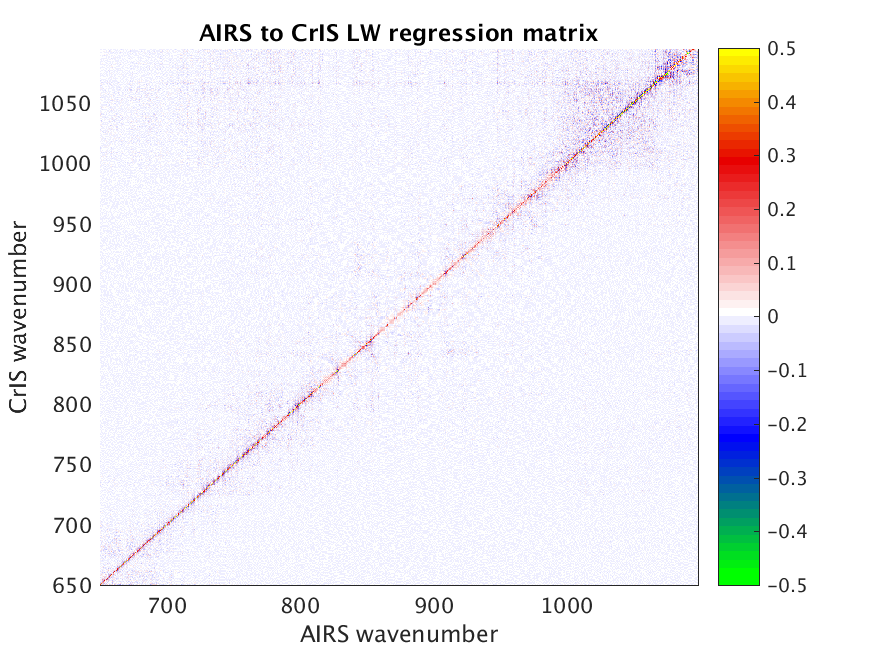
\includegraphics[width=\linewidth]{figures/LW_pc_regr_mat.png}
%   \caption{Regression coefficients from the 7377 profile dependent
%     set for LW principal component regression with $i = j = 500$.}
%   \label{dreg7}
% \end{figure}

\begin{figure} % source slackfigs a2cris_regr5X.m
  \centering
  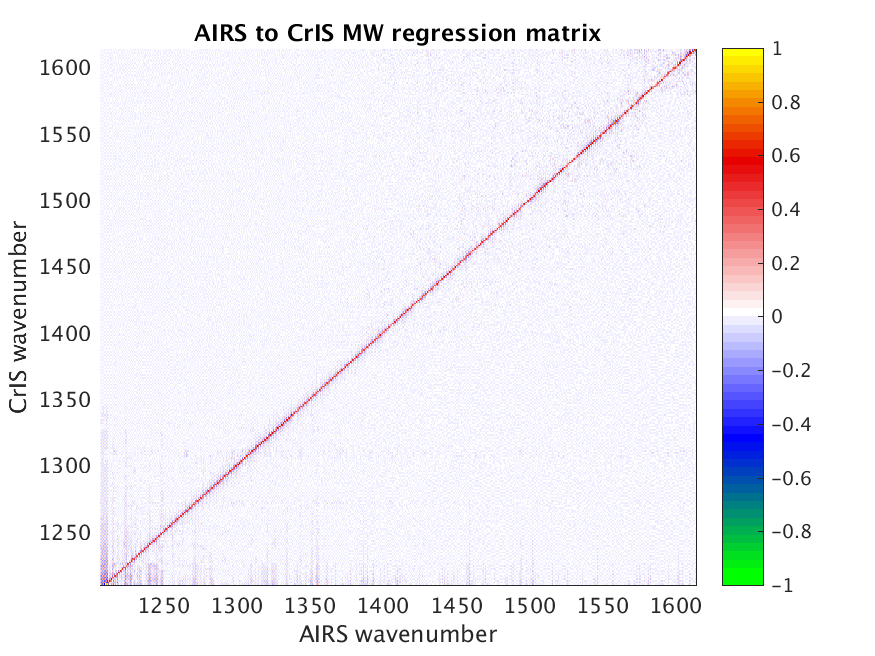
\includegraphics[width=\linewidth]{figures/MW_pc_regr_mat.png}
  \caption{Regression transform from the 7377 profile dependent set
    for MW apodized principal component regression with $i = 500$
    and $j = 320$.}
  \label{dreg8}
\end{figure}

% \begin{figure} % source slackfigs a2cris_regr5.m
%   \centering
%   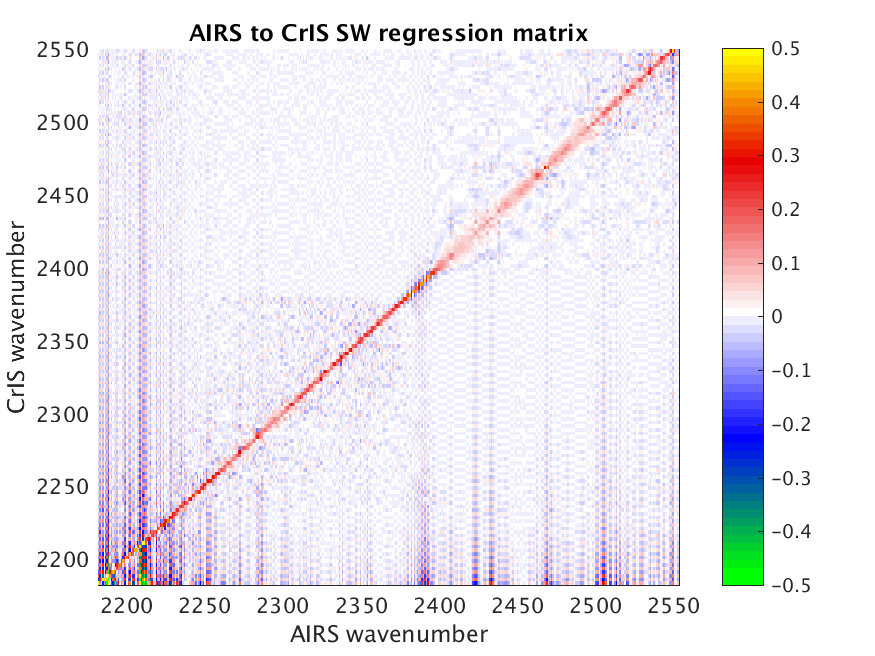
\includegraphics[width=\linewidth]{figures/SW_pc_regr_mat.png}
%   \caption{Regression coefficients from the 7377 profile dependent
%     set for SW principal component regression with $i = j = 100$.}
%   \label{dreg9}
% \end{figure}

% As an alternative we tried a form of principal component regression.

Common techniques for reducing such correlation include adding
noise, restricting the solution to a banded matrix, or working with
principal component decompositions of the data.  We had best results
with the latter.  As above let $r_a$ and $r_c$ be $m \times k$ and
$n \times k$ {\airs} and {\cris} radiance sets.  Let $r_a = U_a
S_a\,V_a^T$ be the singular value decomposition with singular values
in descending order and $U_a^i$ the first $i$ columns of $U_a$.
Similarly let $r_c = U_c S_c\,V_c^T$ be a singular value
decomposition with singular values in descending order and $U_c^j$
the first $j$ columns of $U_c$.  Let $\hat r_a = (U_a^i)^T r_a$ and
$\hat r_c = (U_c^j)^T r_c$ be $r_a$ and $r_c$ represented with
respect to the bases $U_a^i$ and $U_c^j$.  (Since the bases are
orthonormal, the transpose is the inverse.)  Then as before find $X$
by regression to minimize $\|X \hat r_a - \hat r_c\|_2$.  This gives
us $R = U_c^j X (U_a^i)^T$, an {\airs} to {\cris} transform
parameterized by the basis sizes $i$ and $j$.

% Then as before find $X$ to minimize $\|X \hat r_a - \hat r_c\|_2$
% by solving $\hat r_a^T X^T = \hat r_c^T$ for $X$ by regression.

Note that our principal component regression is not the same as
regression after principal component (or singular vector) filtering;
for that we would take $\bar r_a = U_a^i (U_a^i)^T r_a$, $\bar r_c =
U_c^j (U_c^j)^T r_c$, find $X$ to minimize $\|X \bar r_a - \bar
r_c\|_2$, and have no need for a change of bases to apply $X$.  In
practice this did not work as well as doing regression after the
change of bases.

% Figure \ref{dreg6} shows residuals and figures \ref{dreg7},
% \ref{dreg8}, and \ref{dreg9} the transform $R$ for the {\cris} LW,
% MW, and SW bands.  

Figure \ref{dreg6} shows residuals and figure \ref{dreg8} the
transform $R$ for the {\cris} MW band.  We have chosen $i = j = 500$
for the LW, $i = 500$ and $j = 320$ for the MW, and $i = j = 100$
for the SW for the basis sizes, to roughly balance unwanted
correlation with residual size.  The off-diagonal correlations are
significantly reduced, but the residuals are now larger than for the
deconvolution-based translation summarized in figure \ref{statAll1}.
We conclude that principal component regression works fairly well,
in comparison with regular regression or interpolation, but not
quite as well as the deconvolution-based translation.

%---------------------------------------------------------------------
% \FloatBarrier
\section{Applications}  
\label{appcon}

We have been using the {\airs} to {\cris} and {\iasi} to {\cris}
translations to analyze simultaneous nadir overpasses (SNOs)
\cite{wang2015, sno1} and hope to create a long-term climate record
spanning observations from multiple sounders.  The translation of
response functions as discussed here is just one part of such a
project.  To build a common record we must choose a target format.
This might be CrIS standard resolution, a CrIS intermediate
resolution as proposed in section \ref{airs2cris}, or the
generalized Gaussian basis of section \ref{airsL1d}.  The choice
constrains which sounders or resolution modes can be included.  For
example, our proposed {\cris} 0.8/0.6/0.4 \wn\ intermediate
resolution would mean dropping two and a half years (April 2012 to
November 2014) of overlap of AIRS and CrIS standard resolution data.
This sort of problem is inherent in building a common record---over
time resolving power and band spans typically increase.  But a
target format is constrained by what is available from the start.

Uniform spatial sampling is a key part of a long-term record.
{\airs} and {\cris} sampling is similar but not identical.  Details
are beyond the scope of this paper, but some subsetting is typically
necessary.  For example most of our sampling analysis is downstream
from a ``latitude weighted subset'', the selection of all
observations such that $X < |\cos(\hbox{latitude})|$, where $X$ is a
random variable from the uniform distribution $[0, 1]$
\cite{git:acsamp}.  Further subsetting, to correct for sampling
biases or simply to save space, may be desirable.

For some applications these translations allow the use of a common
radiative transfer model and retrieval algorithm.  For applications
such as assimilation and physical retrievals the translation would
need added noise, as discussed in section \ref{airs2cris}.  Finally,
a possible future application is to revisit the {\airs} SRF
measurements, to see if adjustments (within the original measurement
uncertainty) can reduce the translation residuals.

% Given the work that goes into developing and refining models, that
% could be a significant advantage.

% \FloatBarrier
\section{Appendix}
\label{append}

\subsection{Measures of correlation}

We want to measure the correlation of a set of radiances.  One such
measure is dimension of a spanning set.  For an approximation we use
the basis size needed to get reconstruction residuals below some
fixed threshold.  Let $r_0$ be an $m \times n$ array of radiances,
one row per channel and one column per observation.  Let $r_1 = U
S\,V^T$ be a singular value decomposition with singular values in
descending order and $U_k$ the first $k$ columns of $U$.  Let $r_k =
U_k U_k^T r_0$; then $r_k \approx r_0$.  The approximation improves
as $k$ increases and becomes exact for some $k <= m$.  This is the
analog of principal component filtering using left-singular rather
than eigenvectors and is useful as a form of compression when $k$ is
small relative to $n$.  For that case we save $U_k$ and $U_k^T r_0$
separately.  Applications include compression of IASI radiance data
and the {\kcarta} absorption coefficient database.

We use a threshold for equivalence that is relevant for our
applications.  Let $B^{-1}$ be the inverse Planck function and
define $d(r_1, r_2) = \rms(B^{-1}(r_1, v) - B^{-1}(r_2, v))$, the
{\rms} difference over all channels and observations of the
brightness temperatures of radiance data.  Finally let $j$ be the
smallest value such that $d(r_0, r_j) \le T_d$, for some threshold
$T_d$.  Then $j$ is the effective dimension of our set $r_0$.  Here
we have chosen $T_d = 0.02$~K.  For the 49 profile fitting set this
gives $j=48$, which we interpret as largely uncorrelated, while for
the 7377 profile cloudy set we found $j=260$, which we interpret as
highly correlated.

\subsection{Conventional interpolation}
\label{interp}

The {\airs} to {\cris} translation via deconvolution works
significantly better than conventional interpolation.  This is not
surprising since the former makes use of both the source and target
response functions.  We consider two cases.  For the first, start
with true {\airs} and interpolate radiances directly to the {\cris}
user grid with a cubic spline.  This makes no use of either the
{\airs} or {\cris} response functions.  For the second, interpolate
true {\airs} to the 0.1 {\wn} intermediate grid with a cubic spline
and then convolve this to the {\cris} user grid.  This uses the
{\cris} but not the {\airs} response functions.  Results for
apodized {\cris} LW radiance are summarized in Figure~\ref{intpLW}.
As expected, residuals for spline interpolation alone are larger
that for spline interpolation followed by convolution to the {\cris}
user grid, and both are significantly larger than residuals for
{\airs} deconvolution followed by the {\cris} convolution.  Results
for the MW and SW are similar.

\begin{figure} % source a2cris_test1
  \centering
  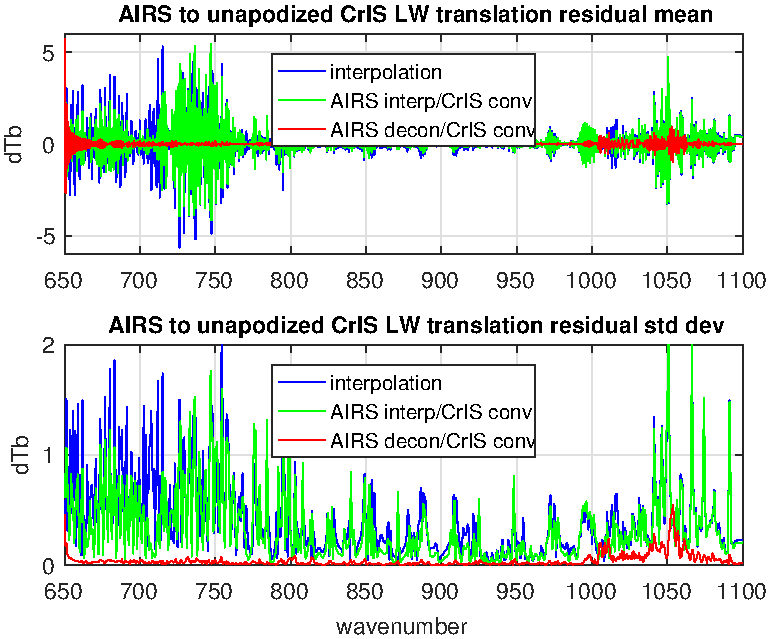
\includegraphics[width=\linewidth]{figures/a2cris_interp_LW.pdf}
  \caption{The AIRS to apodized CrIS translation via spline
    interpolation, interpolation followed by CrIS convolution, and AIRS
    deconvolution followed by CrIS convolution.}
  \label{intpLW}
\end{figure}

\begin{figure} % source L1d_test2.m
  \centering
  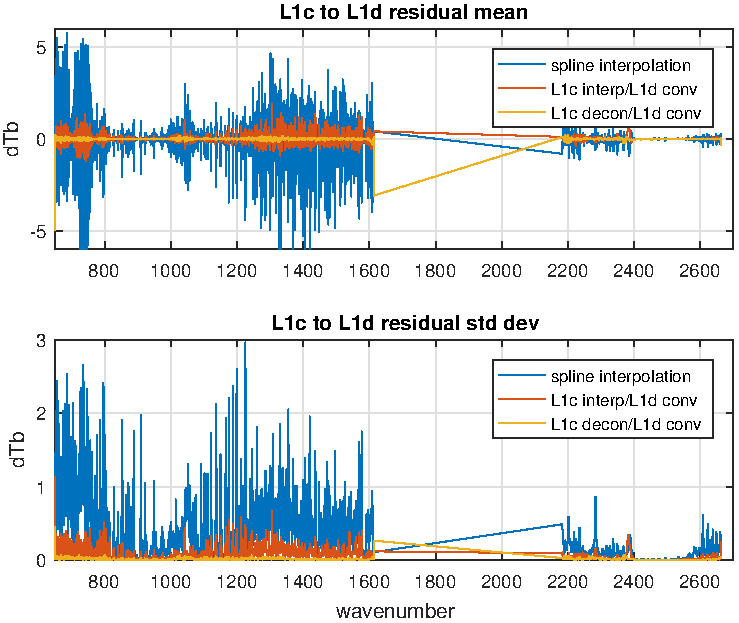
\includegraphics[width=\linewidth]{figures/CtoD_interp_diff.pdf}
  \caption{The AIRS L1c to L1d translation via spline interpolation,
    interpolation followed by CrIS convolution, and AIRS
    deconvolution followed by CrIS convolution.}
  \label{interpL1d}
\end{figure}

The {\airs} L1c to L1d translation via deconvolution also works
significantly better than interpolation.  As before, we consider 
two cases.  For the first, start with true {\airs} and interpolate
radiances directly to the L1d grid with a cubic spline.  For the
second, interpolate true {\airs} to the 0.1 {\wn} intermediate grid
with a cubic spline and convolve this to the L1d channel set.
Results for a resolving power of 700 are summarized in
Figure~\ref{interpL1d}.  Residuals for spline interpolation are
larger that for spline interpolation followed by convolution to the
L1d channel set, and both are significantly larger than residuals
for {\airs} deconvolution followed by the L1d convolution.

\subsection{Source code}

Matlab code for the translations and tests described here (including
the {\iasi} to {\cris}, {\iasi} to {\airs}, and {\cris} to {\airs}
translations mentioned in the introduction) is available at GitHub:

\begin{itemize}
%  \item \url{https://github.com/motteler/decon_paper}
   \item \url{https://github.com/strow/airs_deconv}
   \item \url{https://github.com/strow/iasi_decon}
\end{itemize}

The translations have been tested extensively.  Runtime for the
{\airs} to {\cris} translation is split fairly evenly between
deconvolution and reconvolution.  It takes about 30 seconds to
translate our 7377 profile cloudy set running on one processor.
Calculating the pseudo-inverse adds another 10 seconds, but that
only needs to be done when the translation parameters change.

% The translations can be explicit or implicit---that is, run once
% and saved as a dataset, or run as needed on existing data.

% \FloatBarrier
% \bibliographystyle{abbrv}
% \bibliography{decon_paper}
\bibliographystyle{IEEEtran}
\bibliography{IEEEabrv,decon_paper}

% received the B.S. degree in mathematics from the University of Puget
% Sound, Tacoma, Washington, in 1980, an M.S. in computer science from
% Purdue University, West Lafayette, Indiana, in 1983, and

% hack for bio spacing
% \vspace{10cm}\vfill

\begin{IEEEbiography}[{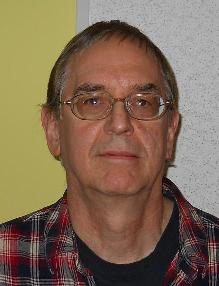
\includegraphics[width=1in,height=1.25in,clip,keepaspectratio]{motte.jpg}}]{Howard~E.~Motteler}
  (M~'87) received the Ph.D. degree in computer science from the
  University of Maryland at College Park in 1987.  From 1987 to 1994
  he was an Assistant Professor and from 1994 to 1998 an Associate
  Professor of computer science at the University of Maryland
  Baltimore County, and from 1992 to 1993 an NRC Research Associate
  at NASA/GSFC.  Since 1998 (with a break from 2008 to 2011) he has
  been a Research Associate Professor at the Joint Center for Earth
  Systems Technology, Baltimore MD.  His research interests include
  infrared sounder modeling and calibration and analysis of AIRS and
  CrIS data for validation and trending.

\end{IEEEbiography}

% hack for bio spacing
% \vspace{-14cm}

\begin{IEEEbiography}[{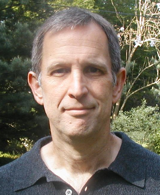
\includegraphics[width=1in,height=1.25in,clip,keepaspectratio]{strow.jpg}}]{L.~Larrabee~Strow}
  received the Ph.D. degree in physics from the University of
  Maryland, College Park, in 1981. He is currently a Research
  Professor with the Department of Physics, University of Maryland
  Baltimore County, Baltimore, MD. His work focuses on remote
  sensing of the Earth in the infrared using high spectral
  resolution satellite instruments. His primary goal is to measure
  climate trends using infrared sensors flown by NASA, NOAA, and
  EUMETSAT. To that end, he is a Science Team Member of NASA’s Aqua
  Atmospheric InfraRed Sounder (AIRS) instrument, the
  NPOESS/JPSS(NOAA-20) Cross-track Infrared Sounder (CrIS) and
  EUMETSAT's Infrared Atmospheric Sounding Interferometer (IASI).
  He also provides NASA and NOAA with the radiative transfer
  algorithms for the retrieval of geophysical variable using AIRS,
  IASI, and CrIS.
\end{IEEEbiography}

\end{document}

